\documentclass[1p]{elsarticle_modified}
%\bibliographystyle{elsarticle-num}

%\usepackage[colorlinks]{hyperref}
%\usepackage{abbrmath_seonhwa} %\Abb, \Ascr, \Acal ,\Abf, \Afrak
\usepackage{amsfonts}
\usepackage{amssymb}
\usepackage{amsmath}
\usepackage{amsthm}
\usepackage{scalefnt}
\usepackage{amsbsy}
\usepackage{kotex}
\usepackage{caption}
\usepackage{subfig}
\usepackage{color}
\usepackage{graphicx}
\usepackage{xcolor} %% white, black, red, green, blue, cyan, magenta, yellow
\usepackage{float}
\usepackage{setspace}
\usepackage{hyperref}

\usepackage{tikz}
\usetikzlibrary{arrows}

\usepackage{multirow}
\usepackage{array} % fixed length table
\usepackage{hhline}

%%%%%%%%%%%%%%%%%%%%%
\makeatletter
\renewcommand*\env@matrix[1][\arraystretch]{%
	\edef\arraystretch{#1}%
	\hskip -\arraycolsep
	\let\@ifnextchar\new@ifnextchar
	\array{*\c@MaxMatrixCols c}}
\makeatother %https://tex.stackexchange.com/questions/14071/how-can-i-increase-the-line-spacing-in-a-matrix
%%%%%%%%%%%%%%%

\usepackage[normalem]{ulem}

\newcommand{\msout}[1]{\ifmmode\text{\sout{\ensuremath{#1}}}\else\sout{#1}\fi}
%SOURCE: \msout is \stkout macro in https://tex.stackexchange.com/questions/20609/strikeout-in-math-mode

\newcommand{\cancel}[1]{
	\ifmmode
	{\color{red}\msout{#1}}
	\else
	{\color{red}\sout{#1}}
	\fi
}

\newcommand{\add}[1]{
	{\color{blue}\uwave{#1}}
}

\newcommand{\replace}[2]{
	\ifmmode
	{\color{red}\msout{#1}}{\color{blue}\uwave{#2}}
	\else
	{\color{red}\sout{#1}}{\color{blue}\uwave{#2}}
	\fi
}

\newcommand{\Sol}{\mathcal{S}} %segment
\newcommand{\D}{D} %diagram
\newcommand{\A}{\mathcal{A}} %arc


%%%%%%%%%%%%%%%%%%%%%%%%%%%%%5 test

\def\sl{\operatorname{\textup{SL}}(2,\Cbb)}
\def\psl{\operatorname{\textup{PSL}}(2,\Cbb)}
\def\quan{\mkern 1mu \triangleright \mkern 1mu}

\theoremstyle{definition}
\newtheorem{thm}{Theorem}[section]
\newtheorem{prop}[thm]{Proposition}
\newtheorem{lem}[thm]{Lemma}
\newtheorem{ques}[thm]{Question}
\newtheorem{cor}[thm]{Corollary}
\newtheorem{defn}[thm]{Definition}
\newtheorem{exam}[thm]{Example}
\newtheorem{rmk}[thm]{Remark}
\newtheorem{alg}[thm]{Algorithm}

\newcommand{\I}{\sqrt{-1}}
\begin{document}

%\begin{frontmatter}
%
%\title{Boundary parabolic representations of knots up to 8 crossings}
%
%%% Group authors per affiliation:
%\author{Yunhi Cho} 
%\address{Department of Mathematics, University of Seoul, Seoul, Korea}
%\ead{yhcho@uos.ac.kr}
%
%
%\author{Seonhwa Kim} %\fnref{s_kim}}
%\address{Center for Geometry and Physics, Institute for Basic Science, Pohang, 37673, Korea}
%\ead{ryeona17@ibs.re.kr}
%
%\author{Hyuk Kim}
%\address{Department of Mathematical Sciences, Seoul National University, Seoul 08826, Korea}
%\ead{hyukkim@snu.ac.kr}
%
%\author{Seokbeom Yoon}
%\address{Department of Mathematical Sciences, Seoul National University, Seoul, 08826,  Korea}
%\ead{sbyoon15@snu.ac.kr}
%
%\begin{abstract}
%We find all boundary parabolic representation of knots up to 8 crossings.
%
%\end{abstract}
%\begin{keyword}
%    \MSC[2010] 57M25 
%\end{keyword}
%
%\end{frontmatter}

%\linenumbers
%\tableofcontents
%
\newcommand\colored[1]{\textcolor{white}{\rule[-0.35ex]{0.8em}{1.4ex}}\kern-0.8em\color{red} #1}%
%\newcommand\colored[1]{\textcolor{white}{ #1}\kern-2.17ex	\textcolor{white}{ #1}\kern-1.81ex	\textcolor{white}{ #1}\kern-2.15ex\color{red}#1	}

{\Large $\underline{12a_{0986}~(K12a_{0986})}$}

\setlength{\tabcolsep}{10pt}
\renewcommand{\arraystretch}{1.6}
\vspace{1cm}\begin{tabular}{m{100pt}>{\centering\arraybackslash}m{274pt}}
\multirow{5}{120pt}{
	\centering
	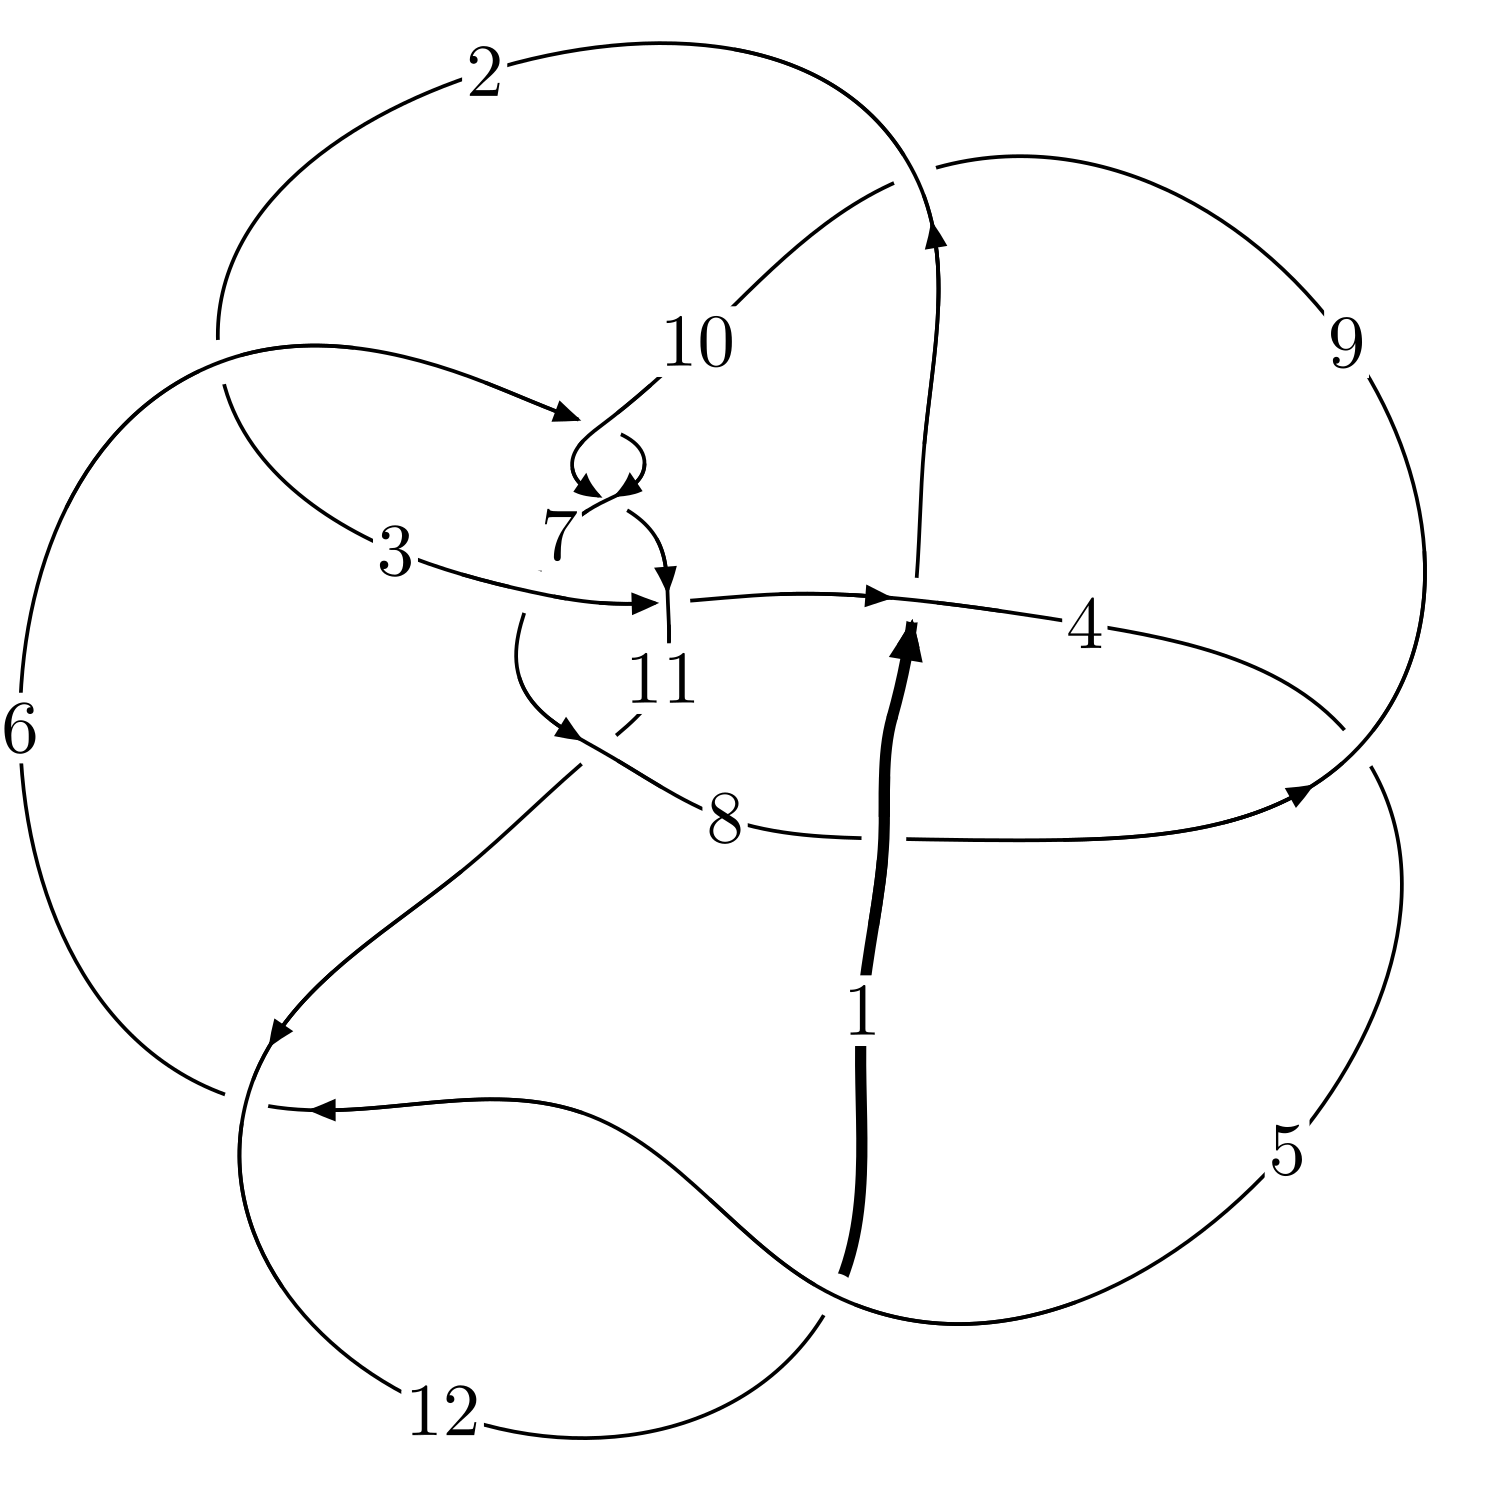
\includegraphics[width=112pt]{../../../GIT/diagram.site/Diagrams/png/1787_12a_0986.png}\\
\ \ \ A knot diagram\footnotemark}&
\allowdisplaybreaks
\textbf{Linearized knot diagam} \\
\cline{2-2}
 &
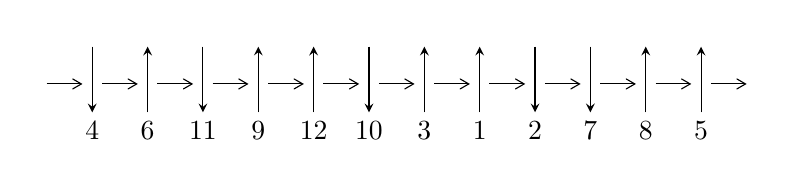
\begin{tikzpicture}[x=20pt, y=17pt]
	% nodes
	\node (C0) at (0, 0) {};
	\node (C1) at (1, 0) {};
	\node (C1U) at (1, +1) {};
	\node (C1D) at (1, -1) {4};

	\node (C2) at (2, 0) {};
	\node (C2U) at (2, +1) {};
	\node (C2D) at (2, -1) {6};

	\node (C3) at (3, 0) {};
	\node (C3U) at (3, +1) {};
	\node (C3D) at (3, -1) {11};

	\node (C4) at (4, 0) {};
	\node (C4U) at (4, +1) {};
	\node (C4D) at (4, -1) {9};

	\node (C5) at (5, 0) {};
	\node (C5U) at (5, +1) {};
	\node (C5D) at (5, -1) {12};

	\node (C6) at (6, 0) {};
	\node (C6U) at (6, +1) {};
	\node (C6D) at (6, -1) {10};

	\node (C7) at (7, 0) {};
	\node (C7U) at (7, +1) {};
	\node (C7D) at (7, -1) {3};

	\node (C8) at (8, 0) {};
	\node (C8U) at (8, +1) {};
	\node (C8D) at (8, -1) {1};

	\node (C9) at (9, 0) {};
	\node (C9U) at (9, +1) {};
	\node (C9D) at (9, -1) {2};

	\node (C10) at (10, 0) {};
	\node (C10U) at (10, +1) {};
	\node (C10D) at (10, -1) {7};

	\node (C11) at (11, 0) {};
	\node (C11U) at (11, +1) {};
	\node (C11D) at (11, -1) {8};

	\node (C12) at (12, 0) {};
	\node (C12U) at (12, +1) {};
	\node (C12D) at (12, -1) {5};
	\node (C13) at (13, 0) {};

	% arrows
	\draw[->,>={angle 60}]
	(C0) edge (C1) (C1) edge (C2) (C2) edge (C3) (C3) edge (C4) (C4) edge (C5) (C5) edge (C6) (C6) edge (C7) (C7) edge (C8) (C8) edge (C9) (C9) edge (C10) (C10) edge (C11) (C11) edge (C12) (C12) edge (C13) ;	\draw[->,>=stealth]
	(C1U) edge (C1D) (C2D) edge (C2U) (C3U) edge (C3D) (C4D) edge (C4U) (C5D) edge (C5U) (C6U) edge (C6D) (C7D) edge (C7U) (C8D) edge (C8U) (C9U) edge (C9D) (C10U) edge (C10D) (C11D) edge (C11U) (C12D) edge (C12U) ;
	\end{tikzpicture} \\
\hhline{~~} \\& 
\textbf{Solving Sequence} \\ \cline{2-2} 
 &
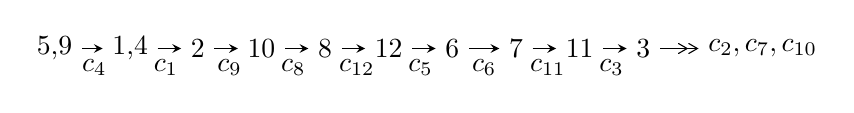
\begin{tikzpicture}[x=23pt, y=7pt]
	% node
	\node (A0) at (-1/8, 0) {5,9};
	\node (A1) at (17/16, 0) {1,4};
	\node (A2) at (17/8, 0) {2};
	\node (A3) at (25/8, 0) {10};
	\node (A4) at (33/8, 0) {8};
	\node (A5) at (41/8, 0) {12};
	\node (A6) at (49/8, 0) {6};
	\node (A7) at (57/8, 0) {7};
	\node (A8) at (65/8, 0) {11};
	\node (A9) at (73/8, 0) {3};
	\node (C1) at (1/2, -1) {$c_{4}$};
	\node (C2) at (13/8, -1) {$c_{1}$};
	\node (C3) at (21/8, -1) {$c_{9}$};
	\node (C4) at (29/8, -1) {$c_{8}$};
	\node (C5) at (37/8, -1) {$c_{12}$};
	\node (C6) at (45/8, -1) {$c_{5}$};
	\node (C7) at (53/8, -1) {$c_{6}$};
	\node (C8) at (61/8, -1) {$c_{11}$};
	\node (C9) at (69/8, -1) {$c_{3}$};
	\node (A10) at (11, 0) {$c_{2},c_{7},c_{10}$};

	% edge
	\draw[->,>=stealth]	
	(A0) edge (A1) (A1) edge (A2) (A2) edge (A3) (A3) edge (A4) (A4) edge (A5) (A5) edge (A6) (A6) edge (A7) (A7) edge (A8) (A8) edge (A9) ;
	\draw[->>,>={angle 60}]	
	(A9) edge (A10);
\end{tikzpicture} \\ 

\end{tabular} \\

\footnotetext{
The image of knot diagram is generated by the software ``\textbf{Draw programme}" developed by Andrew Bartholomew(\url{http://www.layer8.co.uk/maths/draw/index.htm\#Running-draw}), where we modified some parts for our purpose(\url{https://github.com/CATsTAILs/LinksPainter}).
}\phantom \\ \newline 
\centering \textbf{Ideals for irreducible components\footnotemark of $X_{\text{par}}$} 
 
\begin{align*}
I^u_{1}&=\langle 
-6.16032\times10^{1762} u^{178}+3.80838\times10^{1763} u^{177}+\cdots+2.93106\times10^{1765} b+4.85246\times10^{1767},\\
\phantom{I^u_{1}}&\phantom{= \langle  }8.04735\times10^{1767} u^{178}-5.89284\times10^{1768} u^{177}+\cdots+4.20909\times10^{1770} a-4.89264\times10^{1773},\\
\phantom{I^u_{1}}&\phantom{= \langle  }u^{179}-6 u^{178}+\cdots+3332308 u+143603\rangle \\
I^u_{2}&=\langle 
1.58028\times10^{71} u^{37}-1.25122\times10^{72} u^{36}+\cdots+8.18656\times10^{70} b-6.54536\times10^{70},\\
\phantom{I^u_{2}}&\phantom{= \langle  }-1.34545\times10^{71} u^{37}+1.10860\times10^{72} u^{36}+\cdots+8.18656\times10^{70} a-3.01667\times10^{70},\;u^{38}-8 u^{37}+\cdots-4 u+1\rangle \\
I^u_{3}&=\langle 
b-1,\;a-1,\;u+1\rangle \\
\\
\end{align*}
\raggedright * 3 irreducible components of $\dim_{\mathbb{C}}=0$, with total 218 representations.\\
\footnotetext{All coefficients of polynomials are rational numbers. But the coefficients are sometimes approximated in decimal forms when there is not enough margin.}
\newpage
\renewcommand{\arraystretch}{1}
\centering \section*{I. $I^u_{1}= \langle -6.16\times10^{1762} u^{178}+3.81\times10^{1763} u^{177}+\cdots+2.93\times10^{1765} b+4.85\times10^{1767},\;8.05\times10^{1767} u^{178}-5.89\times10^{1768} u^{177}+\cdots+4.21\times10^{1770} a-4.89\times10^{1773},\;u^{179}-6 u^{178}+\cdots+3332308 u+143603 \rangle$}
\flushleft \textbf{(i) Arc colorings}\\
\begin{tabular}{m{7pt} m{180pt} m{7pt} m{180pt} }
\flushright $a_{5}=$&$\begin{pmatrix}1\\0\end{pmatrix}$ \\
\flushright $a_{9}=$&$\begin{pmatrix}0\\u\end{pmatrix}$ \\
\flushright $a_{1}=$&$\begin{pmatrix}-0.00191189 u^{178}+0.0140002 u^{177}+\cdots+25714.7 u+1162.40\\0.00210174 u^{178}-0.0129932 u^{177}+\cdots-2880.36 u-165.553\end{pmatrix}$ \\
\flushright $a_{4}=$&$\begin{pmatrix}1\\u^2\end{pmatrix}$ \\
\flushright $a_{2}=$&$\begin{pmatrix}-0.00362383 u^{178}+0.0239895 u^{177}+\cdots+20442.6 u+964.794\\0.00262200 u^{178}-0.0160995 u^{177}+\cdots-1693.49 u-125.000\end{pmatrix}$ \\
\flushright $a_{10}=$&$\begin{pmatrix}0.000560316 u^{178}-0.00665043 u^{177}+\cdots-34425.1 u-1510.23\\0.000666376 u^{178}-0.00328777 u^{177}+\cdots+7566.53 u+313.227\end{pmatrix}$ \\
\flushright $a_{8}=$&$\begin{pmatrix}0.00225971 u^{178}-0.0169670 u^{177}+\cdots-37421.7 u-1666.78\\0.000291099 u^{178}-0.000834068 u^{177}+\cdots+11351.3 u+491.976\end{pmatrix}$ \\
\flushright $a_{12}=$&$\begin{pmatrix}-0.00401363 u^{178}+0.0269934 u^{177}+\cdots+28595.0 u+1327.95\\0.00210174 u^{178}-0.0129932 u^{177}+\cdots-2880.36 u-165.553\end{pmatrix}$ \\
\flushright $a_{6}=$&$\begin{pmatrix}-0.00329141 u^{178}+0.0203786 u^{177}+\cdots+4078.11 u+241.868\\-0.000134538 u^{178}+0.000468165 u^{177}+\cdots-7028.29 u-306.850\end{pmatrix}$ \\
\flushright $a_{7}=$&$\begin{pmatrix}0.00230578 u^{178}-0.00747566 u^{177}+\cdots+63208.7 u+2747.75\\0.0000421842 u^{178}-0.00240519 u^{177}+\cdots-20941.9 u-916.337\end{pmatrix}$ \\
\flushright $a_{11}=$&$\begin{pmatrix}0.00816482 u^{178}-0.0435919 u^{177}+\cdots+65996.2 u+2760.94\\-0.00154549 u^{178}+0.00740747 u^{177}+\cdots-20350.2 u-859.050\end{pmatrix}$ \\
\flushright $a_{3}=$&$\begin{pmatrix}-0.00317833 u^{178}+0.0165419 u^{177}+\cdots-28787.5 u-1172.32\\-0.000889275 u^{178}+0.00398717 u^{177}+\cdots-11948.1 u-518.874\end{pmatrix}$\\&\end{tabular}
\flushleft \textbf{(ii) Obstruction class $= -1$}\\~\\
\flushleft \textbf{(iii) Cusp Shapes $= 0.00403368 u^{178}-0.0412426 u^{177}+\cdots-165161. u-7415.37$}\\~\\
\newpage\renewcommand{\arraystretch}{1}
\flushleft \textbf{(iv) u-Polynomials at the component}\newline \\
\begin{tabular}{m{50pt}|m{274pt}}
Crossings & \hspace{64pt}u-Polynomials at each crossing \\
\hline $$\begin{aligned}c_{1}\end{aligned}$$&$\begin{aligned}
&u^{179}+13 u^{178}+\cdots+4864 u-127
\end{aligned}$\\
\hline $$\begin{aligned}c_{2}\end{aligned}$$&$\begin{aligned}
&u^{179}+2 u^{178}+\cdots-32727793 u-7268479
\end{aligned}$\\
\hline $$\begin{aligned}c_{3}\end{aligned}$$&$\begin{aligned}
&u^{179}+2 u^{178}+\cdots+8231201 u-980023
\end{aligned}$\\
\hline $$\begin{aligned}c_{4}\end{aligned}$$&$\begin{aligned}
&u^{179}-6 u^{178}+\cdots+3332308 u+143603
\end{aligned}$\\
\hline $$\begin{aligned}c_{5},c_{12}\end{aligned}$$&$\begin{aligned}
&u^{179}+4 u^{178}+\cdots-956262 u-23017
\end{aligned}$\\
\hline $$\begin{aligned}c_{6},c_{10}\end{aligned}$$&$\begin{aligned}
&u^{179}+u^{178}+\cdots-12744 u-496
\end{aligned}$\\
\hline $$\begin{aligned}c_{7}\end{aligned}$$&$\begin{aligned}
&u^{179}-6 u^{178}+\cdots-683 u-29
\end{aligned}$\\
\hline $$\begin{aligned}c_{8}\end{aligned}$$&$\begin{aligned}
&u^{179}-5 u^{178}+\cdots+1340 u+173
\end{aligned}$\\
\hline $$\begin{aligned}c_{9}\end{aligned}$$&$\begin{aligned}
&u^{179}-14 u^{178}+\cdots-56730382524 u+17613549763
\end{aligned}$\\
\hline $$\begin{aligned}c_{11}\end{aligned}$$&$\begin{aligned}
&u^{179}+4 u^{178}+\cdots-2349183 u+256397
\end{aligned}$\\
\hline
\end{tabular}\\~\\
\newpage\renewcommand{\arraystretch}{1}
\flushleft \textbf{(v) Riley Polynomials at the component}\newline \\
\begin{tabular}{m{50pt}|m{274pt}}
Crossings & \hspace{64pt}Riley Polynomials at each crossing \\
\hline $$\begin{aligned}c_{1}\end{aligned}$$&$\begin{aligned}
&y^{179}+y^{178}+\cdots+344852 y-16129
\end{aligned}$\\
\hline $$\begin{aligned}c_{2}\end{aligned}$$&$\begin{aligned}
&y^{179}+66 y^{178}+\cdots-4439617469518745 y-52830786973441
\end{aligned}$\\
\hline $$\begin{aligned}c_{3}\end{aligned}$$&$\begin{aligned}
&y^{179}-20 y^{178}+\cdots+76198792323071 y-960445080529
\end{aligned}$\\
\hline $$\begin{aligned}c_{4}\end{aligned}$$&$\begin{aligned}
&y^{179}+16 y^{178}+\cdots+4839426567530 y-20621821609
\end{aligned}$\\
\hline $$\begin{aligned}c_{5},c_{12}\end{aligned}$$&$\begin{aligned}
&y^{179}+134 y^{178}+\cdots-31322218488 y-529782289
\end{aligned}$\\
\hline $$\begin{aligned}c_{6},c_{10}\end{aligned}$$&$\begin{aligned}
&y^{179}-127 y^{178}+\cdots+4324416 y-246016
\end{aligned}$\\
\hline $$\begin{aligned}c_{7}\end{aligned}$$&$\begin{aligned}
&y^{179}+26 y^{178}+\cdots+119939 y-841
\end{aligned}$\\
\hline $$\begin{aligned}c_{8}\end{aligned}$$&$\begin{aligned}
&y^{179}+5 y^{178}+\cdots+505366 y-29929
\end{aligned}$\\
\hline $$\begin{aligned}c_{9}\end{aligned}$$&$\begin{aligned}
&y^{179}-82 y^{178}+\cdots+2.94\times10^{22} y-3.10\times10^{20}
\end{aligned}$\\
\hline $$\begin{aligned}c_{11}\end{aligned}$$&$\begin{aligned}
&y^{179}+2 y^{178}+\cdots+106182658357 y-65739421609
\end{aligned}$\\
\hline
\end{tabular}\\~\\
\newpage\flushleft \textbf{(vi) Complex Volumes and Cusp Shapes}
$$\begin{array}{c|c|c}  
\text{Solutions to }I^u_{1}& \I (\text{vol} + \sqrt{-1}CS) & \text{Cusp shape}\\
 \hline 
\begin{aligned}
u &= \phantom{-}0.160093 + 0.972700 I \\
a &= \phantom{-}0.497860 - 0.221762 I \\
b &= \phantom{-}0.24369 + 1.57387 I\end{aligned}
 & -9.74999 + 5.34481 I & \phantom{-0.000000 } 0 \\ \hline\begin{aligned}
u &= \phantom{-}0.160093 - 0.972700 I \\
a &= \phantom{-}0.497860 + 0.221762 I \\
b &= \phantom{-}0.24369 - 1.57387 I\end{aligned}
 & -9.74999 - 5.34481 I & \phantom{-0.000000 } 0 \\ \hline\begin{aligned}
u &= \phantom{-}0.863307 + 0.475681 I \\
a &= \phantom{-}0.928468 - 0.222692 I \\
b &= \phantom{-}0.864974 + 0.099404 I\end{aligned}
 & \phantom{-}1.89841 + 0.80237 I & \phantom{-0.000000 } 0 \\ \hline\begin{aligned}
u &= \phantom{-}0.863307 - 0.475681 I \\
a &= \phantom{-}0.928468 + 0.222692 I \\
b &= \phantom{-}0.864974 - 0.099404 I\end{aligned}
 & \phantom{-}1.89841 - 0.80237 I & \phantom{-0.000000 } 0 \\ \hline\begin{aligned}
u &= \phantom{-}0.227170 + 0.958236 I \\
a &= -1.93322 + 0.31633 I \\
b &= -0.075295 - 1.082210 I\end{aligned}
 & -8.76330 + 0.54002 I & \phantom{-0.000000 } 0 \\ \hline\begin{aligned}
u &= \phantom{-}0.227170 - 0.958236 I \\
a &= -1.93322 - 0.31633 I \\
b &= -0.075295 + 1.082210 I\end{aligned}
 & -8.76330 - 0.54002 I & \phantom{-0.000000 } 0 \\ \hline\begin{aligned}
u &= \phantom{-}0.348586 + 0.914122 I \\
a &= -0.904818 - 0.130769 I \\
b &= -0.682093 + 0.168984 I\end{aligned}
 & -5.84833 + 2.26700 I & \phantom{-0.000000 } 0 \\ \hline\begin{aligned}
u &= \phantom{-}0.348586 - 0.914122 I \\
a &= -0.904818 + 0.130769 I \\
b &= -0.682093 - 0.168984 I\end{aligned}
 & -5.84833 - 2.26700 I & \phantom{-0.000000 } 0 \\ \hline\begin{aligned}
u &= \phantom{-}0.688741 + 0.761648 I \\
a &= \phantom{-}0.793429 + 0.812658 I \\
b &= -0.237171 + 0.302856 I\end{aligned}
 & \phantom{-}0.13597 + 4.18324 I & \phantom{-0.000000 } 0 \\ \hline\begin{aligned}
u &= \phantom{-}0.688741 - 0.761648 I \\
a &= \phantom{-}0.793429 - 0.812658 I \\
b &= -0.237171 - 0.302856 I\end{aligned}
 & \phantom{-}0.13597 - 4.18324 I & \phantom{-0.000000 } 0\\
 \hline 
 \end{array}$$\newpage$$\begin{array}{c|c|c}  
\text{Solutions to }I^u_{1}& \I (\text{vol} + \sqrt{-1}CS) & \text{Cusp shape}\\
 \hline 
\begin{aligned}
u &= -0.586776 + 0.848662 I \\
a &= \phantom{-}0.855948 - 0.230798 I \\
b &= \phantom{-}1.075910 - 0.491601 I\end{aligned}
 & -5.35007 + 4.67966 I & \phantom{-0.000000 } 0 \\ \hline\begin{aligned}
u &= -0.586776 - 0.848662 I \\
a &= \phantom{-}0.855948 + 0.230798 I \\
b &= \phantom{-}1.075910 + 0.491601 I\end{aligned}
 & -5.35007 - 4.67966 I & \phantom{-0.000000 } 0 \\ \hline\begin{aligned}
u &= -1.029700 + 0.074717 I \\
a &= \phantom{-}0.516386 - 0.085250 I \\
b &= \phantom{-}0.585551 - 0.946540 I\end{aligned}
 & -0.19117 - 4.10195 I & \phantom{-0.000000 } 0 \\ \hline\begin{aligned}
u &= -1.029700 - 0.074717 I \\
a &= \phantom{-}0.516386 + 0.085250 I \\
b &= \phantom{-}0.585551 + 0.946540 I\end{aligned}
 & -0.19117 + 4.10195 I & \phantom{-0.000000 } 0 \\ \hline\begin{aligned}
u &= \phantom{-}0.940780 + 0.190478 I \\
a &= \phantom{-}0.530871 - 0.009582 I \\
b &= \phantom{-}0.679166 + 0.453939 I\end{aligned}
 & \phantom{-}1.47853 + 0.54393 I & \phantom{-0.000000 } 0 \\ \hline\begin{aligned}
u &= \phantom{-}0.940780 - 0.190478 I \\
a &= \phantom{-}0.530871 + 0.009582 I \\
b &= \phantom{-}0.679166 - 0.453939 I\end{aligned}
 & \phantom{-}1.47853 - 0.54393 I & \phantom{-0.000000 } 0 \\ \hline\begin{aligned}
u &= \phantom{-}0.764943 + 0.575286 I \\
a &= -1.340030 + 0.054344 I \\
b &= -0.770866 + 0.090952 I\end{aligned}
 & \phantom{-}1.56692 + 7.67371 I & \phantom{-0.000000 } 0 \\ \hline\begin{aligned}
u &= \phantom{-}0.764943 - 0.575286 I \\
a &= -1.340030 - 0.054344 I \\
b &= -0.770866 - 0.090952 I\end{aligned}
 & \phantom{-}1.56692 - 7.67371 I & \phantom{-0.000000 } 0 \\ \hline\begin{aligned}
u &= \phantom{-}0.073797 + 0.951967 I \\
a &= \phantom{-}0.74633 - 1.54134 I \\
b &= \phantom{-}0.02008 + 1.47450 I\end{aligned}
 & -9.46264 + 6.62769 I & \phantom{-0.000000 } 0 \\ \hline\begin{aligned}
u &= \phantom{-}0.073797 - 0.951967 I \\
a &= \phantom{-}0.74633 + 1.54134 I \\
b &= \phantom{-}0.02008 - 1.47450 I\end{aligned}
 & -9.46264 - 6.62769 I & \phantom{-0.000000 } 0\\
 \hline 
 \end{array}$$\newpage$$\begin{array}{c|c|c}  
\text{Solutions to }I^u_{1}& \I (\text{vol} + \sqrt{-1}CS) & \text{Cusp shape}\\
 \hline 
\begin{aligned}
u &= \phantom{-}0.824716 + 0.644514 I \\
a &= -1.70775 - 0.44370 I \\
b &= -0.361480 - 1.272120 I\end{aligned}
 & \phantom{-}0.43653 + 7.24900 I & \phantom{-0.000000 } 0 \\ \hline\begin{aligned}
u &= \phantom{-}0.824716 - 0.644514 I \\
a &= -1.70775 + 0.44370 I \\
b &= -0.361480 + 1.272120 I\end{aligned}
 & \phantom{-}0.43653 - 7.24900 I & \phantom{-0.000000 } 0 \\ \hline\begin{aligned}
u &= \phantom{-}0.776001 + 0.713953 I \\
a &= \phantom{-}0.849169 + 0.087983 I \\
b &= \phantom{-}1.205560 + 0.550268 I\end{aligned}
 & \phantom{-}0.561818 + 0.664728 I & \phantom{-0.000000 } 0 \\ \hline\begin{aligned}
u &= \phantom{-}0.776001 - 0.713953 I \\
a &= \phantom{-}0.849169 - 0.087983 I \\
b &= \phantom{-}1.205560 - 0.550268 I\end{aligned}
 & \phantom{-}0.561818 - 0.664728 I & \phantom{-0.000000 } 0 \\ \hline\begin{aligned}
u &= -0.599781 + 0.715422 I \\
a &= \phantom{-}0.311755 + 0.775076 I \\
b &= -0.0814523 - 0.1124140 I\end{aligned}
 & -3.06266 + 0.89643 I & \phantom{-0.000000 } 0 \\ \hline\begin{aligned}
u &= -0.599781 - 0.715422 I \\
a &= \phantom{-}0.311755 - 0.775076 I \\
b &= -0.0814523 + 0.1124140 I\end{aligned}
 & -3.06266 - 0.89643 I & \phantom{-0.000000 } 0 \\ \hline\begin{aligned}
u &= \phantom{-}0.212812 + 1.054210 I \\
a &= -1.203940 - 0.064128 I \\
b &= -0.500082 - 1.157870 I\end{aligned}
 & -9.23720 + 1.61235 I & \phantom{-0.000000 } 0 \\ \hline\begin{aligned}
u &= \phantom{-}0.212812 - 1.054210 I \\
a &= -1.203940 + 0.064128 I \\
b &= -0.500082 + 1.157870 I\end{aligned}
 & -9.23720 - 1.61235 I & \phantom{-0.000000 } 0 \\ \hline\begin{aligned}
u &= -0.193163 + 0.900694 I \\
a &= \phantom{-}1.66089 + 0.96416 I \\
b &= -0.239455 - 1.137520 I\end{aligned}
 & -6.08490 - 0.22834 I & \phantom{-0.000000 } 0 \\ \hline\begin{aligned}
u &= -0.193163 - 0.900694 I \\
a &= \phantom{-}1.66089 - 0.96416 I \\
b &= -0.239455 + 1.137520 I\end{aligned}
 & -6.08490 + 0.22834 I & \phantom{-0.000000 } 0\\
 \hline 
 \end{array}$$\newpage$$\begin{array}{c|c|c}  
\text{Solutions to }I^u_{1}& \I (\text{vol} + \sqrt{-1}CS) & \text{Cusp shape}\\
 \hline 
\begin{aligned}
u &= -0.102826 + 0.911024 I \\
a &= \phantom{-}1.282050 + 0.116325 I \\
b &= \phantom{-}0.70598 - 1.37876 I\end{aligned}
 & -8.2321 - 11.6976 I & \phantom{-0.000000 } 0 \\ \hline\begin{aligned}
u &= -0.102826 - 0.911024 I \\
a &= \phantom{-}1.282050 - 0.116325 I \\
b &= \phantom{-}0.70598 + 1.37876 I\end{aligned}
 & -8.2321 + 11.6976 I & \phantom{-0.000000 } 0 \\ \hline\begin{aligned}
u &= \phantom{-}0.830316 + 0.695838 I \\
a &= \phantom{-}0.727043 - 0.294344 I \\
b &= \phantom{-}0.673614 + 0.444373 I\end{aligned}
 & \phantom{-}1.50907 + 0.82449 I & \phantom{-0.000000 } 0 \\ \hline\begin{aligned}
u &= \phantom{-}0.830316 - 0.695838 I \\
a &= \phantom{-}0.727043 + 0.294344 I \\
b &= \phantom{-}0.673614 - 0.444373 I\end{aligned}
 & \phantom{-}1.50907 - 0.82449 I & \phantom{-0.000000 } 0 \\ \hline\begin{aligned}
u &= \phantom{-}0.256033 + 0.866301 I \\
a &= -0.962825 - 0.132000 I \\
b &= -0.676501 + 1.021890 I\end{aligned}
 & -6.62253 + 2.55245 I & \phantom{-0.000000 } 0 \\ \hline\begin{aligned}
u &= \phantom{-}0.256033 - 0.866301 I \\
a &= -0.962825 + 0.132000 I \\
b &= -0.676501 - 1.021890 I\end{aligned}
 & -6.62253 - 2.55245 I & \phantom{-0.000000 } 0 \\ \hline\begin{aligned}
u &= \phantom{-}0.915606 + 0.613815 I \\
a &= \phantom{-}1.019860 + 0.042862 I \\
b &= \phantom{-}0.494658 + 1.320780 I\end{aligned}
 & -2.45085 + 5.31363 I & \phantom{-0.000000 } 0 \\ \hline\begin{aligned}
u &= \phantom{-}0.915606 - 0.613815 I \\
a &= \phantom{-}1.019860 - 0.042862 I \\
b &= \phantom{-}0.494658 - 1.320780 I\end{aligned}
 & -2.45085 - 5.31363 I & \phantom{-0.000000 } 0 \\ \hline\begin{aligned}
u &= -0.768277 + 0.808272 I \\
a &= \phantom{-}1.58099 + 0.02550 I \\
b &= \phantom{-}0.369712 - 1.036040 I\end{aligned}
 & -0.672545 - 0.169536 I & \phantom{-0.000000 } 0 \\ \hline\begin{aligned}
u &= -0.768277 - 0.808272 I \\
a &= \phantom{-}1.58099 - 0.02550 I \\
b &= \phantom{-}0.369712 + 1.036040 I\end{aligned}
 & -0.672545 + 0.169536 I & \phantom{-0.000000 } 0\\
 \hline 
 \end{array}$$\newpage$$\begin{array}{c|c|c}  
\text{Solutions to }I^u_{1}& \I (\text{vol} + \sqrt{-1}CS) & \text{Cusp shape}\\
 \hline 
\begin{aligned}
u &= -0.163103 + 0.853775 I \\
a &= -0.472117 + 1.142500 I \\
b &= \phantom{-}0.027335 - 1.135330 I\end{aligned}
 & -3.17479 - 1.74755 I & \phantom{-0.000000 } 0 \\ \hline\begin{aligned}
u &= -0.163103 - 0.853775 I \\
a &= -0.472117 - 1.142500 I \\
b &= \phantom{-}0.027335 + 1.135330 I\end{aligned}
 & -3.17479 + 1.74755 I & \phantom{-0.000000 } 0 \\ \hline\begin{aligned}
u &= \phantom{-}0.639061 + 0.587893 I \\
a &= \phantom{-}1.325060 - 0.451588 I \\
b &= \phantom{-}0.634750 - 0.485703 I\end{aligned}
 & \phantom{-}1.03467 - 3.77002 I & \phantom{-0.000000 } 0 \\ \hline\begin{aligned}
u &= \phantom{-}0.639061 - 0.587893 I \\
a &= \phantom{-}1.325060 + 0.451588 I \\
b &= \phantom{-}0.634750 + 0.485703 I\end{aligned}
 & \phantom{-}1.03467 + 3.77002 I & \phantom{-0.000000 } 0 \\ \hline\begin{aligned}
u &= -0.877697 + 0.715406 I \\
a &= -0.609623 - 0.059229 I \\
b &= -1.347230 - 0.074470 I\end{aligned}
 & \phantom{-}0.88251 - 1.57486 I & \phantom{-0.000000 } 0 \\ \hline\begin{aligned}
u &= -0.877697 - 0.715406 I \\
a &= -0.609623 + 0.059229 I \\
b &= -1.347230 + 0.074470 I\end{aligned}
 & \phantom{-}0.88251 + 1.57486 I & \phantom{-0.000000 } 0 \\ \hline\begin{aligned}
u &= -0.812606 + 0.805228 I \\
a &= \phantom{-}0.707262 - 0.850886 I \\
b &= -0.132813 - 0.364925 I\end{aligned}
 & -4.76824 - 9.86796 I & \phantom{-0.000000 } 0 \\ \hline\begin{aligned}
u &= -0.812606 - 0.805228 I \\
a &= \phantom{-}0.707262 + 0.850886 I \\
b &= -0.132813 + 0.364925 I\end{aligned}
 & -4.76824 + 9.86796 I & \phantom{-0.000000 } 0 \\ \hline\begin{aligned}
u &= \phantom{-}0.030914 + 0.850026 I \\
a &= -1.44184 - 0.41331 I \\
b &= -0.040538 + 1.166310 I\end{aligned}
 & -7.37766 + 3.47007 I & \phantom{-0.000000 } 0 \\ \hline\begin{aligned}
u &= \phantom{-}0.030914 - 0.850026 I \\
a &= -1.44184 + 0.41331 I \\
b &= -0.040538 - 1.166310 I\end{aligned}
 & -7.37766 - 3.47007 I & \phantom{-0.000000 } 0\\
 \hline 
 \end{array}$$\newpage$$\begin{array}{c|c|c}  
\text{Solutions to }I^u_{1}& \I (\text{vol} + \sqrt{-1}CS) & \text{Cusp shape}\\
 \hline 
\begin{aligned}
u &= \phantom{-}0.505194 + 0.668862 I \\
a &= \phantom{-}1.032550 - 0.146240 I \\
b &= \phantom{-}1.48308 - 0.33304 I\end{aligned}
 & -2.42701 + 0.79923 I & \phantom{-0.000000 } 0 \\ \hline\begin{aligned}
u &= \phantom{-}0.505194 - 0.668862 I \\
a &= \phantom{-}1.032550 + 0.146240 I \\
b &= \phantom{-}1.48308 + 0.33304 I\end{aligned}
 & -2.42701 - 0.79923 I & \phantom{-0.000000 } 0 \\ \hline\begin{aligned}
u &= \phantom{-}0.698233 + 0.945327 I \\
a &= -0.853474 + 0.250990 I \\
b &= -0.893587 - 0.022074 I\end{aligned}
 & \phantom{-}0.58797 + 4.89617 I & \phantom{-0.000000 } 0 \\ \hline\begin{aligned}
u &= \phantom{-}0.698233 - 0.945327 I \\
a &= -0.853474 - 0.250990 I \\
b &= -0.893587 + 0.022074 I\end{aligned}
 & \phantom{-}0.58797 - 4.89617 I & \phantom{-0.000000 } 0 \\ \hline\begin{aligned}
u &= -0.834787 + 0.828542 I \\
a &= \phantom{-}0.897864 + 0.098076 I \\
b &= \phantom{-}1.337730 - 0.113546 I\end{aligned}
 & \phantom{-}2.36439 - 8.92822 I & \phantom{-0.000000 } 0 \\ \hline\begin{aligned}
u &= -0.834787 - 0.828542 I \\
a &= \phantom{-}0.897864 - 0.098076 I \\
b &= \phantom{-}1.337730 + 0.113546 I\end{aligned}
 & \phantom{-}2.36439 + 8.92822 I & \phantom{-0.000000 } 0 \\ \hline\begin{aligned}
u &= \phantom{-}0.790379 + 0.875687 I \\
a &= \phantom{-}1.352410 + 0.052564 I \\
b &= \phantom{-}0.506007 + 1.045380 I\end{aligned}
 & \phantom{-}2.14555 + 4.55407 I & \phantom{-0.000000 } 0 \\ \hline\begin{aligned}
u &= \phantom{-}0.790379 - 0.875687 I \\
a &= \phantom{-}1.352410 - 0.052564 I \\
b &= \phantom{-}0.506007 - 1.045380 I\end{aligned}
 & \phantom{-}2.14555 - 4.55407 I & \phantom{-0.000000 } 0 \\ \hline\begin{aligned}
u &= -0.585447 + 0.573438 I \\
a &= -0.552705 + 0.603540 I \\
b &= -0.362732 - 0.270376 I\end{aligned}
 & -1.32808 - 1.47127 I & \phantom{-0.000000 } 0 \\ \hline\begin{aligned}
u &= -0.585447 - 0.573438 I \\
a &= -0.552705 - 0.603540 I \\
b &= -0.362732 + 0.270376 I\end{aligned}
 & -1.32808 + 1.47127 I & \phantom{-0.000000 } 0\\
 \hline 
 \end{array}$$\newpage$$\begin{array}{c|c|c}  
\text{Solutions to }I^u_{1}& \I (\text{vol} + \sqrt{-1}CS) & \text{Cusp shape}\\
 \hline 
\begin{aligned}
u &= \phantom{-}0.997414 + 0.657988 I \\
a &= -0.057148 - 0.577116 I \\
b &= -0.187606 + 0.345330 I\end{aligned}
 & -3.54281 + 1.91947 I & \phantom{-0.000000 } 0 \\ \hline\begin{aligned}
u &= \phantom{-}0.997414 - 0.657988 I \\
a &= -0.057148 + 0.577116 I \\
b &= -0.187606 - 0.345330 I\end{aligned}
 & -3.54281 - 1.91947 I & \phantom{-0.000000 } 0 \\ \hline\begin{aligned}
u &= -0.686884 + 0.985272 I \\
a &= -0.323542 - 0.286212 I \\
b &= -0.317306 - 0.660641 I\end{aligned}
 & -1.18591 - 5.40154 I & \phantom{-0.000000 } 0 \\ \hline\begin{aligned}
u &= -0.686884 - 0.985272 I \\
a &= -0.323542 + 0.286212 I \\
b &= -0.317306 + 0.660641 I\end{aligned}
 & -1.18591 + 5.40154 I & \phantom{-0.000000 } 0 \\ \hline\begin{aligned}
u &= -1.158180 + 0.349051 I \\
a &= \phantom{-}0.186684 + 0.320600 I \\
b &= \phantom{-}0.209073 + 1.061440 I\end{aligned}
 & -0.96105 + 2.77423 I & \phantom{-0.000000 } 0 \\ \hline\begin{aligned}
u &= -1.158180 - 0.349051 I \\
a &= \phantom{-}0.186684 - 0.320600 I \\
b &= \phantom{-}0.209073 - 1.061440 I\end{aligned}
 & -0.96105 - 2.77423 I & \phantom{-0.000000 } 0 \\ \hline\begin{aligned}
u &= -0.760355 + 0.951557 I \\
a &= -0.908322 - 0.055771 I \\
b &= -0.882253 - 0.098344 I\end{aligned}
 & -3.37196 - 6.50628 I & \phantom{-0.000000 } 0 \\ \hline\begin{aligned}
u &= -0.760355 - 0.951557 I \\
a &= -0.908322 + 0.055771 I \\
b &= -0.882253 + 0.098344 I\end{aligned}
 & -3.37196 + 6.50628 I & \phantom{-0.000000 } 0 \\ \hline\begin{aligned}
u &= -0.549885 + 0.554076 I \\
a &= \phantom{-}1.233420 + 0.321718 I \\
b &= \phantom{-}0.873176 + 0.431306 I\end{aligned}
 & \phantom{-}4.12918 + 0.46038 I & \phantom{-0.000000 } 0 \\ \hline\begin{aligned}
u &= -0.549885 - 0.554076 I \\
a &= \phantom{-}1.233420 - 0.321718 I \\
b &= \phantom{-}0.873176 - 0.431306 I\end{aligned}
 & \phantom{-}4.12918 - 0.46038 I & \phantom{-0.000000 } 0\\
 \hline 
 \end{array}$$\newpage$$\begin{array}{c|c|c}  
\text{Solutions to }I^u_{1}& \I (\text{vol} + \sqrt{-1}CS) & \text{Cusp shape}\\
 \hline 
\begin{aligned}
u &= -0.178864 + 0.752610 I \\
a &= -1.67611 + 0.14821 I \\
b &= -0.462338 + 1.173420 I\end{aligned}
 & -4.75246 - 1.54481 I & \phantom{-0.000000 } 0 \\ \hline\begin{aligned}
u &= -0.178864 - 0.752610 I \\
a &= -1.67611 - 0.14821 I \\
b &= -0.462338 - 1.173420 I\end{aligned}
 & -4.75246 + 1.54481 I & \phantom{-0.000000 } 0 \\ \hline\begin{aligned}
u &= \phantom{-}0.200263 + 0.731281 I \\
a &= \phantom{-}1.304330 - 0.105083 I \\
b &= \phantom{-}0.65375 + 1.47229 I\end{aligned}
 & -2.80609 + 7.16976 I & \phantom{-0.000000 } 0 \\ \hline\begin{aligned}
u &= \phantom{-}0.200263 - 0.731281 I \\
a &= \phantom{-}1.304330 + 0.105083 I \\
b &= \phantom{-}0.65375 - 1.47229 I\end{aligned}
 & -2.80609 - 7.16976 I & \phantom{-0.000000 } 0 \\ \hline\begin{aligned}
u &= -0.830272 + 0.923562 I \\
a &= \phantom{-}1.102330 - 0.171863 I \\
b &= \phantom{-}0.814467 - 0.884213 I\end{aligned}
 & -3.92574 - 8.99449 I & \phantom{-0.000000 } 0 \\ \hline\begin{aligned}
u &= -0.830272 - 0.923562 I \\
a &= \phantom{-}1.102330 + 0.171863 I \\
b &= \phantom{-}0.814467 + 0.884213 I\end{aligned}
 & -3.92574 + 8.99449 I & \phantom{-0.000000 } 0 \\ \hline\begin{aligned}
u &= -0.209625 + 0.728236 I \\
a &= -1.96239 - 0.96863 I \\
b &= -0.372436 + 1.359620 I\end{aligned}
 & -6.87153 - 4.30366 I & \phantom{-0.000000 } 0 \\ \hline\begin{aligned}
u &= -0.209625 - 0.728236 I \\
a &= -1.96239 + 0.96863 I \\
b &= -0.372436 - 1.359620 I\end{aligned}
 & -6.87153 + 4.30366 I & \phantom{-0.000000 } 0 \\ \hline\begin{aligned}
u &= \phantom{-}0.833955 + 0.923717 I \\
a &= \phantom{-}0.889138 - 0.119543 I \\
b &= \phantom{-}1.286160 + 0.053699 I\end{aligned}
 & -2.6444 + 14.9286 I & \phantom{-0.000000 } 0 \\ \hline\begin{aligned}
u &= \phantom{-}0.833955 - 0.923717 I \\
a &= \phantom{-}0.889138 + 0.119543 I \\
b &= \phantom{-}1.286160 - 0.053699 I\end{aligned}
 & -2.6444 - 14.9286 I & \phantom{-0.000000 } 0\\
 \hline 
 \end{array}$$\newpage$$\begin{array}{c|c|c}  
\text{Solutions to }I^u_{1}& \I (\text{vol} + \sqrt{-1}CS) & \text{Cusp shape}\\
 \hline 
\begin{aligned}
u &= \phantom{-}0.778610 + 0.973425 I \\
a &= -0.037400 + 0.233340 I \\
b &= -0.261633 + 0.643199 I\end{aligned}
 & \phantom{-}1.93607 + 1.35235 I & \phantom{-0.000000 } 0 \\ \hline\begin{aligned}
u &= \phantom{-}0.778610 - 0.973425 I \\
a &= -0.037400 - 0.233340 I \\
b &= -0.261633 - 0.643199 I\end{aligned}
 & \phantom{-}1.93607 - 1.35235 I & \phantom{-0.000000 } 0 \\ \hline\begin{aligned}
u &= -0.478419 + 1.159430 I \\
a &= -0.716340 - 0.504402 I \\
b &= -0.769362 + 0.163942 I\end{aligned}
 & -2.11487 - 5.21570 I & \phantom{-0.000000 } 0 \\ \hline\begin{aligned}
u &= -0.478419 - 1.159430 I \\
a &= -0.716340 + 0.504402 I \\
b &= -0.769362 - 0.163942 I\end{aligned}
 & -2.11487 + 5.21570 I & \phantom{-0.000000 } 0 \\ \hline\begin{aligned}
u &= -0.207889 + 0.713914 I \\
a &= \phantom{-}1.72989 + 1.73093 I \\
b &= -0.024620 - 1.340490 I\end{aligned}
 & -4.44495 - 1.81498 I & \phantom{-0.000000 } 0 \\ \hline\begin{aligned}
u &= -0.207889 - 0.713914 I \\
a &= \phantom{-}1.72989 - 1.73093 I \\
b &= -0.024620 + 1.340490 I\end{aligned}
 & -4.44495 + 1.81498 I & \phantom{-0.000000 } 0 \\ \hline\begin{aligned}
u &= -0.714841 + 1.033450 I \\
a &= \phantom{-}0.500873 - 0.521611 I \\
b &= -0.314896 - 0.564591 I\end{aligned}
 & -4.19245 + 2.74490 I & \phantom{-0.000000 } 0 \\ \hline\begin{aligned}
u &= -0.714841 - 1.033450 I \\
a &= \phantom{-}0.500873 + 0.521611 I \\
b &= -0.314896 + 0.564591 I\end{aligned}
 & -4.19245 - 2.74490 I & \phantom{-0.000000 } 0 \\ \hline\begin{aligned}
u &= -0.889537 + 0.918502 I \\
a &= \phantom{-}1.049510 + 0.121298 I \\
b &= \phantom{-}0.471707 - 1.329920 I\end{aligned}
 & -2.47079 - 5.72434 I & \phantom{-0.000000 } 0 \\ \hline\begin{aligned}
u &= -0.889537 - 0.918502 I \\
a &= \phantom{-}1.049510 - 0.121298 I \\
b &= \phantom{-}0.471707 + 1.329920 I\end{aligned}
 & -2.47079 + 5.72434 I & \phantom{-0.000000 } 0\\
 \hline 
 \end{array}$$\newpage$$\begin{array}{c|c|c}  
\text{Solutions to }I^u_{1}& \I (\text{vol} + \sqrt{-1}CS) & \text{Cusp shape}\\
 \hline 
\begin{aligned}
u &= \phantom{-}0.526664 + 0.464979 I \\
a &= -0.34088 + 1.64668 I \\
b &= -0.549169 - 0.227075 I\end{aligned}
 & -2.48389 + 2.59715 I & \phantom{-0.000000 } 0 \\ \hline\begin{aligned}
u &= \phantom{-}0.526664 - 0.464979 I \\
a &= -0.34088 - 1.64668 I \\
b &= -0.549169 + 0.227075 I\end{aligned}
 & -2.48389 - 2.59715 I & \phantom{-0.000000 } 0 \\ \hline\begin{aligned}
u &= -0.555438 + 0.402882 I \\
a &= -1.84210 - 0.20467 I \\
b &= -0.718058 - 0.085859 I\end{aligned}
 & \phantom{-}4.17872 - 3.24163 I & \phantom{-0.000000 } 0 \\ \hline\begin{aligned}
u &= -0.555438 - 0.402882 I \\
a &= -1.84210 + 0.20467 I \\
b &= -0.718058 + 0.085859 I\end{aligned}
 & \phantom{-}4.17872 + 3.24163 I & \phantom{-0.000000 } 0 \\ \hline\begin{aligned}
u &= \phantom{-}0.068096 + 0.666391 I \\
a &= \phantom{-}2.28793 + 2.33841 I \\
b &= -0.185761 - 1.134860 I\end{aligned}
 & -7.14233 + 11.57710 I & \phantom{-0.000000 } 0 \\ \hline\begin{aligned}
u &= \phantom{-}0.068096 - 0.666391 I \\
a &= \phantom{-}2.28793 - 2.33841 I \\
b &= -0.185761 + 1.134860 I\end{aligned}
 & -7.14233 - 11.57710 I & \phantom{-0.000000 } 0 \\ \hline\begin{aligned}
u &= -1.015180 + 0.873522 I \\
a &= -1.288660 + 0.207699 I \\
b &= -0.406918 + 1.260950 I\end{aligned}
 & -2.08717 - 12.02360 I & \phantom{-0.000000 } 0 \\ \hline\begin{aligned}
u &= -1.015180 - 0.873522 I \\
a &= -1.288660 - 0.207699 I \\
b &= -0.406918 - 1.260950 I\end{aligned}
 & -2.08717 + 12.02360 I & \phantom{-0.000000 } 0 \\ \hline\begin{aligned}
u &= \phantom{-}0.022859 + 0.659179 I \\
a &= -2.47200 + 0.40487 I \\
b &= -0.372992 - 1.220430 I\end{aligned}
 & -7.40547 + 0.57805 I & \phantom{-0.000000 } 0 \\ \hline\begin{aligned}
u &= \phantom{-}0.022859 - 0.659179 I \\
a &= -2.47200 - 0.40487 I \\
b &= -0.372992 + 1.220430 I\end{aligned}
 & -7.40547 - 0.57805 I & \phantom{-0.000000 } 0\\
 \hline 
 \end{array}$$\newpage$$\begin{array}{c|c|c}  
\text{Solutions to }I^u_{1}& \I (\text{vol} + \sqrt{-1}CS) & \text{Cusp shape}\\
 \hline 
\begin{aligned}
u &= \phantom{-}0.048055 + 0.652340 I \\
a &= \phantom{-}2.60598 - 1.76336 I \\
b &= -0.191187 + 1.143260 I\end{aligned}
 & -2.41113 - 6.11278 I & \phantom{-0.000000 } 0 \\ \hline\begin{aligned}
u &= \phantom{-}0.048055 - 0.652340 I \\
a &= \phantom{-}2.60598 + 1.76336 I \\
b &= -0.191187 - 1.143260 I\end{aligned}
 & -2.41113 + 6.11278 I & \phantom{-0.000000 } 0 \\ \hline\begin{aligned}
u &= -0.707221 + 1.154200 I \\
a &= -0.154817 - 0.618372 I \\
b &= -0.591930 + 0.497062 I\end{aligned}
 & \phantom{-}1.58908 + 2.85999 I & \phantom{-0.000000 } 0 \\ \hline\begin{aligned}
u &= -0.707221 - 1.154200 I \\
a &= -0.154817 + 0.618372 I \\
b &= -0.591930 - 0.497062 I\end{aligned}
 & \phantom{-}1.58908 - 2.85999 I & \phantom{-0.000000 } 0 \\ \hline\begin{aligned}
u &= \phantom{-}0.917364 + 1.013270 I \\
a &= -0.347413 + 0.657807 I \\
b &= -0.663798 - 0.433140 I\end{aligned}
 & -2.70586 - 8.47057 I & \phantom{-0.000000 } 0 \\ \hline\begin{aligned}
u &= \phantom{-}0.917364 - 1.013270 I \\
a &= -0.347413 - 0.657807 I \\
b &= -0.663798 + 0.433140 I\end{aligned}
 & -2.70586 + 8.47057 I & \phantom{-0.000000 } 0 \\ \hline\begin{aligned}
u &= -0.927664 + 1.004460 I \\
a &= \phantom{-}0.577050 + 0.308715 I \\
b &= \phantom{-}0.776435 - 0.996279 I\end{aligned}
 & -0.06821 - 5.05747 I & \phantom{-0.000000 } 0 \\ \hline\begin{aligned}
u &= -0.927664 - 1.004460 I \\
a &= \phantom{-}0.577050 - 0.308715 I \\
b &= \phantom{-}0.776435 + 0.996279 I\end{aligned}
 & -0.06821 + 5.05747 I & \phantom{-0.000000 } 0 \\ \hline\begin{aligned}
u &= -0.245062 + 0.579462 I \\
a &= -3.67087 - 0.02131 I \\
b &= -0.040610 + 1.052940 I\end{aligned}
 & -4.17418 - 0.33308 I & \phantom{-0.000000 } 0 \\ \hline\begin{aligned}
u &= -0.245062 - 0.579462 I \\
a &= -3.67087 + 0.02131 I \\
b &= -0.040610 - 1.052940 I\end{aligned}
 & -4.17418 + 0.33308 I & \phantom{-0.000000 } 0\\
 \hline 
 \end{array}$$\newpage$$\begin{array}{c|c|c}  
\text{Solutions to }I^u_{1}& \I (\text{vol} + \sqrt{-1}CS) & \text{Cusp shape}\\
 \hline 
\begin{aligned}
u &= \phantom{-}0.868708 + 1.063090 I \\
a &= -0.640306 + 0.256969 I \\
b &= -1.027020 - 0.195423 I\end{aligned}
 & \phantom{-}0.36610 + 5.45734 I & \phantom{-0.000000 } 0 \\ \hline\begin{aligned}
u &= \phantom{-}0.868708 - 1.063090 I \\
a &= -0.640306 - 0.256969 I \\
b &= -1.027020 + 0.195423 I\end{aligned}
 & \phantom{-}0.36610 - 5.45734 I & \phantom{-0.000000 } 0 \\ \hline\begin{aligned}
u &= -0.619952 + 0.045093 I \\
a &= \phantom{-}0.03036 + 1.41390 I \\
b &= -0.235997 - 0.092149 I\end{aligned}
 & -1.23428 - 1.94780 I & \phantom{-0.000000 } 0 \\ \hline\begin{aligned}
u &= -0.619952 - 0.045093 I \\
a &= \phantom{-}0.03036 - 1.41390 I \\
b &= -0.235997 + 0.092149 I\end{aligned}
 & -1.23428 + 1.94780 I & \phantom{-0.000000 } 0 \\ \hline\begin{aligned}
u &= -0.151428 + 0.596501 I \\
a &= \phantom{-}0.482224 - 0.229925 I \\
b &= \phantom{-}0.52984 + 1.99627 I\end{aligned}
 & -7.85639 - 7.09052 I & \phantom{-0.000000 } 0 \\ \hline\begin{aligned}
u &= -0.151428 - 0.596501 I \\
a &= \phantom{-}0.482224 + 0.229925 I \\
b &= \phantom{-}0.52984 - 1.99627 I\end{aligned}
 & -7.85639 + 7.09052 I & \phantom{-0.000000 } 0 \\ \hline\begin{aligned}
u &= -0.594618 + 0.119364 I \\
a &= \phantom{-}0.10329 + 2.87694 I \\
b &= -0.112042 + 1.045700 I\end{aligned}
 & -4.08515 + 0.25044 I & \phantom{-0.000000 } 0 \\ \hline\begin{aligned}
u &= -0.594618 - 0.119364 I \\
a &= \phantom{-}0.10329 - 2.87694 I \\
b &= -0.112042 - 1.045700 I\end{aligned}
 & -4.08515 - 0.25044 I & \phantom{-0.000000 } 0 \\ \hline\begin{aligned}
u &= -0.056666 + 0.600305 I \\
a &= -0.895367 + 0.757269 I \\
b &= -0.67891 - 1.49549 I\end{aligned}
 & -2.14404 + 0.79987 I & \phantom{-0.000000 } 0 \\ \hline\begin{aligned}
u &= -0.056666 - 0.600305 I \\
a &= -0.895367 - 0.757269 I \\
b &= -0.67891 + 1.49549 I\end{aligned}
 & -2.14404 - 0.79987 I & \phantom{-0.000000 } 0\\
 \hline 
 \end{array}$$\newpage$$\begin{array}{c|c|c}  
\text{Solutions to }I^u_{1}& \I (\text{vol} + \sqrt{-1}CS) & \text{Cusp shape}\\
 \hline 
\begin{aligned}
u &= \phantom{-}0.593887 + 1.272390 I \\
a &= -1.231230 + 0.507892 I \\
b &= -0.42265 - 1.37452 I\end{aligned}
 & -6.90638 + 9.70537 I & \phantom{-0.000000 } 0 \\ \hline\begin{aligned}
u &= \phantom{-}0.593887 - 1.272390 I \\
a &= -1.231230 - 0.507892 I \\
b &= -0.42265 + 1.37452 I\end{aligned}
 & -6.90638 - 9.70537 I & \phantom{-0.000000 } 0 \\ \hline\begin{aligned}
u &= -0.58949 + 1.29030 I \\
a &= -1.155590 - 0.299227 I \\
b &= -0.086537 + 1.045290 I\end{aligned}
 & -7.02019 - 4.73556 I & \phantom{-0.000000 } 0 \\ \hline\begin{aligned}
u &= -0.58949 - 1.29030 I \\
a &= -1.155590 + 0.299227 I \\
b &= -0.086537 - 1.045290 I\end{aligned}
 & -7.02019 + 4.73556 I & \phantom{-0.000000 } 0 \\ \hline\begin{aligned}
u &= -0.096241 + 0.556917 I \\
a &= -0.18416 - 3.49270 I \\
b &= -0.17002 + 1.42553 I\end{aligned}
 & -7.78381 - 5.08706 I & \phantom{-0.000000 } 0 \\ \hline\begin{aligned}
u &= -0.096241 - 0.556917 I \\
a &= -0.18416 + 3.49270 I \\
b &= -0.17002 - 1.42553 I\end{aligned}
 & -7.78381 + 5.08706 I & \phantom{-0.000000 } 0 \\ \hline\begin{aligned}
u &= -0.88499 + 1.19709 I \\
a &= \phantom{-}1.044950 + 0.081648 I \\
b &= \phantom{-}0.65855 - 1.47534 I\end{aligned}
 & -6.56185 - 8.48761 I & \phantom{-0.000000 } 0 \\ \hline\begin{aligned}
u &= -0.88499 - 1.19709 I \\
a &= \phantom{-}1.044950 - 0.081648 I \\
b &= \phantom{-}0.65855 + 1.47534 I\end{aligned}
 & -6.56185 + 8.48761 I & \phantom{-0.000000 } 0 \\ \hline\begin{aligned}
u &= -0.502578 + 0.029572 I \\
a &= \phantom{-}0.587731 + 0.819387 I \\
b &= -0.923361 + 1.048100 I\end{aligned}
 & -3.18892 + 0.13773 I & \phantom{-0.000000 } 0 \\ \hline\begin{aligned}
u &= -0.502578 - 0.029572 I \\
a &= \phantom{-}0.587731 - 0.819387 I \\
b &= -0.923361 - 1.048100 I\end{aligned}
 & -3.18892 - 0.13773 I & \phantom{-0.000000 } 0\\
 \hline 
 \end{array}$$\newpage$$\begin{array}{c|c|c}  
\text{Solutions to }I^u_{1}& \I (\text{vol} + \sqrt{-1}CS) & \text{Cusp shape}\\
 \hline 
\begin{aligned}
u &= -0.82549 + 1.25389 I \\
a &= -1.115040 - 0.213766 I \\
b &= -0.468214 + 1.319910 I\end{aligned}
 & -3.57182 - 9.85619 I & \phantom{-0.000000 } 0 \\ \hline\begin{aligned}
u &= -0.82549 - 1.25389 I \\
a &= -1.115040 + 0.213766 I \\
b &= -0.468214 - 1.319910 I\end{aligned}
 & -3.57182 + 9.85619 I & \phantom{-0.000000 } 0 \\ \hline\begin{aligned}
u &= \phantom{-}0.374800 + 0.292914 I \\
a &= \phantom{-}6.13466 - 3.18111 I \\
b &= \phantom{-}0.054068 + 0.996470 I\end{aligned}
 & -4.99300 - 0.33552 I & -27.2414 - 41.7810 I \\ \hline\begin{aligned}
u &= \phantom{-}0.374800 - 0.292914 I \\
a &= \phantom{-}6.13466 + 3.18111 I \\
b &= \phantom{-}0.054068 - 0.996470 I\end{aligned}
 & -4.99300 + 0.33552 I & -27.2414 + 41.7810 I \\ \hline\begin{aligned}
u &= -0.77045 + 1.32923 I \\
a &= -0.893629 - 0.033316 I \\
b &= -0.548137 + 1.230160 I\end{aligned}
 & -8.72545 - 7.23788 I & \phantom{-0.000000 } 0 \\ \hline\begin{aligned}
u &= -0.77045 - 1.32923 I \\
a &= -0.893629 + 0.033316 I \\
b &= -0.548137 - 1.230160 I\end{aligned}
 & -8.72545 + 7.23788 I & \phantom{-0.000000 } 0 \\ \hline\begin{aligned}
u &= \phantom{-}0.92726 + 1.28543 I \\
a &= \phantom{-}1.024210 - 0.130374 I \\
b &= \phantom{-}0.58001 + 1.44025 I\end{aligned}
 & -2.4722 + 15.4837 I & \phantom{-0.000000 } 0 \\ \hline\begin{aligned}
u &= \phantom{-}0.92726 - 1.28543 I \\
a &= \phantom{-}1.024210 + 0.130374 I \\
b &= \phantom{-}0.58001 - 1.44025 I\end{aligned}
 & -2.4722 - 15.4837 I & \phantom{-0.000000 } 0 \\ \hline\begin{aligned}
u &= \phantom{-}1.17680 + 1.06498 I \\
a &= -0.490988 - 0.065967 I \\
b &= -0.664865 - 1.096620 I\end{aligned}
 & -1.74065 + 6.08639 I & \phantom{-0.000000 } 0 \\ \hline\begin{aligned}
u &= \phantom{-}1.17680 - 1.06498 I \\
a &= -0.490988 + 0.065967 I \\
b &= -0.664865 + 1.096620 I\end{aligned}
 & -1.74065 - 6.08639 I & \phantom{-0.000000 } 0\\
 \hline 
 \end{array}$$\newpage$$\begin{array}{c|c|c}  
\text{Solutions to }I^u_{1}& \I (\text{vol} + \sqrt{-1}CS) & \text{Cusp shape}\\
 \hline 
\begin{aligned}
u &= \phantom{-}0.310053 + 0.263275 I \\
a &= -0.31163 - 1.92118 I \\
b &= \phantom{-}0.133198 - 1.307840 I\end{aligned}
 & -3.42587 - 5.39201 I & -2.05136 + 9.05405 I \\ \hline\begin{aligned}
u &= \phantom{-}0.310053 - 0.263275 I \\
a &= -0.31163 + 1.92118 I \\
b &= \phantom{-}0.133198 + 1.307840 I\end{aligned}
 & -3.42587 + 5.39201 I & -2.05136 - 9.05405 I \\ \hline\begin{aligned}
u &= \phantom{-}0.32202 + 1.57783 I \\
a &= -0.363831 + 0.860317 I \\
b &= -0.119673 - 1.014670 I\end{aligned}
 & -1.93093 + 7.12112 I & \phantom{-0.000000 } 0 \\ \hline\begin{aligned}
u &= \phantom{-}0.32202 - 1.57783 I \\
a &= -0.363831 - 0.860317 I \\
b &= -0.119673 + 1.014670 I\end{aligned}
 & -1.93093 - 7.12112 I & \phantom{-0.000000 } 0 \\ \hline\begin{aligned}
u &= -0.077935 + 0.377163 I \\
a &= \phantom{-}0.843812 + 0.140353 I \\
b &= \phantom{-}0.16952 - 2.67977 I\end{aligned}
 & -3.36973 - 0.05585 I & -2.6990 - 34.3862 I \\ \hline\begin{aligned}
u &= -0.077935 - 0.377163 I \\
a &= \phantom{-}0.843812 - 0.140353 I \\
b &= \phantom{-}0.16952 + 2.67977 I\end{aligned}
 & -3.36973 + 0.05585 I & -2.6990 + 34.3862 I \\ \hline\begin{aligned}
u &= -0.92363 + 1.33176 I \\
a &= \phantom{-}1.031020 + 0.147555 I \\
b &= \phantom{-}0.57969 - 1.42037 I\end{aligned}
 & -7.2659 - 21.3644 I & \phantom{-0.000000 } 0 \\ \hline\begin{aligned}
u &= -0.92363 - 1.33176 I \\
a &= \phantom{-}1.031020 - 0.147555 I \\
b &= \phantom{-}0.57969 + 1.42037 I\end{aligned}
 & -7.2659 + 21.3644 I & \phantom{-0.000000 } 0 \\ \hline\begin{aligned}
u &= -0.77203 + 1.44418 I \\
a &= -0.887214 - 0.426998 I \\
b &= -0.52175 + 1.41477 I\end{aligned}
 & -4.62617 - 11.08030 I & \phantom{-0.000000 } 0 \\ \hline\begin{aligned}
u &= -0.77203 - 1.44418 I \\
a &= -0.887214 + 0.426998 I \\
b &= -0.52175 - 1.41477 I\end{aligned}
 & -4.62617 + 11.08030 I & \phantom{-0.000000 } 0\\
 \hline 
 \end{array}$$\newpage$$\begin{array}{c|c|c}  
\text{Solutions to }I^u_{1}& \I (\text{vol} + \sqrt{-1}CS) & \text{Cusp shape}\\
 \hline 
\begin{aligned}
u &= \phantom{-}0.87994 + 1.38732 I \\
a &= -0.807919 + 0.228085 I \\
b &= -0.59381 - 1.33204 I\end{aligned}
 & -3.02264 + 8.05656 I & \phantom{-0.000000 } 0 \\ \hline\begin{aligned}
u &= \phantom{-}0.87994 - 1.38732 I \\
a &= -0.807919 - 0.228085 I \\
b &= -0.59381 + 1.33204 I\end{aligned}
 & -3.02264 - 8.05656 I & \phantom{-0.000000 } 0 \\ \hline\begin{aligned}
u &= \phantom{-}0.95370 + 1.33962 I \\
a &= -1.018510 + 0.086896 I \\
b &= -0.486965 - 1.275330 I\end{aligned}
 & -7.03458 + 11.51160 I & \phantom{-0.000000 } 0 \\ \hline\begin{aligned}
u &= \phantom{-}0.95370 - 1.33962 I \\
a &= -1.018510 - 0.086896 I \\
b &= -0.486965 + 1.275330 I\end{aligned}
 & -7.03458 - 11.51160 I & \phantom{-0.000000 } 0 \\ \hline\begin{aligned}
u &= -0.11589 + 1.66220 I \\
a &= -0.053249 - 0.729882 I \\
b &= -0.132085 + 0.983979 I\end{aligned}
 & \phantom{-}1.25928 - 3.20214 I & \phantom{-0.000000 } 0 \\ \hline\begin{aligned}
u &= -0.11589 - 1.66220 I \\
a &= -0.053249 + 0.729882 I \\
b &= -0.132085 - 0.983979 I\end{aligned}
 & \phantom{-}1.25928 + 3.20214 I & \phantom{-0.000000 } 0 \\ \hline\begin{aligned}
u &= -1.57651 + 0.57677 I \\
a &= \phantom{-}0.047699 - 0.384593 I \\
b &= -0.336148 - 0.994125 I\end{aligned}
 & -4.57155 + 0.66290 I & \phantom{-0.000000 } 0 \\ \hline\begin{aligned}
u &= -1.57651 - 0.57677 I \\
a &= \phantom{-}0.047699 + 0.384593 I \\
b &= -0.336148 + 0.994125 I\end{aligned}
 & -4.57155 - 0.66290 I & \phantom{-0.000000 } 0 \\ \hline\begin{aligned}
u &= -0.96790 + 1.37986 I \\
a &= \phantom{-}0.775609 + 0.061189 I \\
b &= \phantom{-}0.27393 - 1.40481 I\end{aligned}
 & -6.16921 - 5.17837 I & \phantom{-0.000000 } 0 \\ \hline\begin{aligned}
u &= -0.96790 - 1.37986 I \\
a &= \phantom{-}0.775609 - 0.061189 I \\
b &= \phantom{-}0.27393 + 1.40481 I\end{aligned}
 & -6.16921 + 5.17837 I & \phantom{-0.000000 } 0\\
 \hline 
 \end{array}$$\newpage$$\begin{array}{c|c|c}  
\text{Solutions to }I^u_{1}& \I (\text{vol} + \sqrt{-1}CS) & \text{Cusp shape}\\
 \hline 
\begin{aligned}
u &= \phantom{-}0.83824 + 1.47663 I \\
a &= \phantom{-}0.722373 - 0.134243 I \\
b &= \phantom{-}0.321672 + 1.368770 I\end{aligned}
 & -11.24820 - 0.45268 I & \phantom{-0.000000 } 0 \\ \hline\begin{aligned}
u &= \phantom{-}0.83824 - 1.47663 I \\
a &= \phantom{-}0.722373 + 0.134243 I \\
b &= \phantom{-}0.321672 - 1.368770 I\end{aligned}
 & -11.24820 + 0.45268 I & \phantom{-0.000000 } 0 \\ \hline\begin{aligned}
u &= \phantom{-}1.15676 + 1.25806 I \\
a &= -0.647712 - 0.164410 I \\
b &= -0.062926 - 1.039870 I\end{aligned}
 & -2.71036 + 2.84323 I & \phantom{-0.000000 } 0 \\ \hline\begin{aligned}
u &= \phantom{-}1.15676 - 1.25806 I \\
a &= -0.647712 + 0.164410 I \\
b &= -0.062926 + 1.039870 I\end{aligned}
 & -2.71036 - 2.84323 I & \phantom{-0.000000 } 0 \\ \hline\begin{aligned}
u &= -0.46140 + 1.73293 I \\
a &= -0.0633685 + 0.1068600 I \\
b &= -0.055244 - 1.113700 I\end{aligned}
 & -2.70384 - 1.58733 I & \phantom{-0.000000 } 0 \\ \hline\begin{aligned}
u &= -0.46140 - 1.73293 I \\
a &= -0.0633685 - 0.1068600 I \\
b &= -0.055244 + 1.113700 I\end{aligned}
 & -2.70384 + 1.58733 I & \phantom{-0.000000 } 0 \\ \hline\begin{aligned}
u &= \phantom{-}1.08708 + 1.48110 I \\
a &= \phantom{-}0.697954 - 0.022329 I \\
b &= \phantom{-}0.245406 + 1.338960 I\end{aligned}
 & -10.3414 + 11.5088 I & \phantom{-0.000000 } 0 \\ \hline\begin{aligned}
u &= \phantom{-}1.08708 - 1.48110 I \\
a &= \phantom{-}0.697954 + 0.022329 I \\
b &= \phantom{-}0.245406 - 1.338960 I\end{aligned}
 & -10.3414 - 11.5088 I & \phantom{-0.000000 } 0 \\ \hline\begin{aligned}
u &= \phantom{-}1.83664 + 0.43092 I \\
a &= -0.111631 + 0.222303 I \\
b &= -0.413025 + 1.029520 I\end{aligned}
 & \phantom{-}0.03047 - 6.88807 I & \phantom{-0.000000 } 0 \\ \hline\begin{aligned}
u &= \phantom{-}1.83664 - 0.43092 I \\
a &= -0.111631 - 0.222303 I \\
b &= -0.413025 - 1.029520 I\end{aligned}
 & \phantom{-}0.03047 + 6.88807 I & \phantom{-0.000000 } 0\\
 \hline 
 \end{array}$$\newpage$$\begin{array}{c|c|c}  
\text{Solutions to }I^u_{1}& \I (\text{vol} + \sqrt{-1}CS) & \text{Cusp shape}\\
 \hline 
\begin{aligned}
u &= -1.87599 + 0.42811 I \\
a &= -0.166649 - 0.224487 I \\
b &= -0.407132 - 1.038160 I\end{aligned}
 & -4.49649 + 12.60060 I & \phantom{-0.000000 } 0 \\ \hline\begin{aligned}
u &= -1.87599 - 0.42811 I \\
a &= -0.166649 + 0.224487 I \\
b &= -0.407132 + 1.038160 I\end{aligned}
 & -4.49649 - 12.60060 I & \phantom{-0.000000 } 0 \\ \hline\begin{aligned}
u &= -0.0586417\phantom{ +0.000000I} \\
a &= \phantom{-}4.90444\phantom{ +0.000000I} \\
b &= \phantom{-}1.35371\phantom{ +0.000000I}\end{aligned}
 & \phantom{-}2.62611\phantom{ +0.000000I} & -31.0140\phantom{ +0.000000I} \\ \hline\begin{aligned}
u &= -0.93568 + 1.71441 I \\
a &= \phantom{-}0.225535 + 0.256238 I \\
b &= -0.039317 - 0.849692 I\end{aligned}
 & -3.47794 + 0.87367 I & \phantom{-0.000000 } 0 \\ \hline\begin{aligned}
u &= -0.93568 - 1.71441 I \\
a &= \phantom{-}0.225535 - 0.256238 I \\
b &= -0.039317 + 0.849692 I\end{aligned}
 & -3.47794 - 0.87367 I & \phantom{-0.000000 } 0 \\ \hline\begin{aligned}
u &= \phantom{-}2.31413 + 1.11090 I \\
a &= \phantom{-}0.0749392 - 0.0682635 I \\
b &= -0.015021 + 0.889766 I\end{aligned}
 & -3.75225 + 2.03920 I & \phantom{-0.000000 } 0 \\ \hline\begin{aligned}
u &= \phantom{-}2.31413 - 1.11090 I \\
a &= \phantom{-}0.0749392 + 0.0682635 I \\
b &= -0.015021 - 0.889766 I\end{aligned}
 & -3.75225 - 2.03920 I & \phantom{-0.000000 } 0 \\ \hline\begin{aligned}
u &= \phantom{-}3.91767 + 0.70198 I \\
a &= \phantom{-}0.0706944 + 0.1039240 I \\
b &= \phantom{-}0.019704 + 1.027180 I\end{aligned}
 & -3.09178 - 2.18952 I & \phantom{-0.000000 } 0 \\ \hline\begin{aligned}
u &= \phantom{-}3.91767 - 0.70198 I \\
a &= \phantom{-}0.0706944 - 0.1039240 I \\
b &= \phantom{-}0.019704 - 1.027180 I\end{aligned}
 & -3.09178 + 2.18952 I & \phantom{-0.000000 } 0\\
 \hline 
 \end{array}$$\newpage\newpage\renewcommand{\arraystretch}{1}
\centering \section*{II. $I^u_{2}= \langle 1.58\times10^{71} u^{37}-1.25\times10^{72} u^{36}+\cdots+8.19\times10^{70} b-6.55\times10^{70},\;-1.35\times10^{71} u^{37}+1.11\times10^{72} u^{36}+\cdots+8.19\times10^{70} a-3.02\times10^{70},\;u^{38}-8 u^{37}+\cdots-4 u+1 \rangle$}
\flushleft \textbf{(i) Arc colorings}\\
\begin{tabular}{m{7pt} m{180pt} m{7pt} m{180pt} }
\flushright $a_{5}=$&$\begin{pmatrix}1\\0\end{pmatrix}$ \\
\flushright $a_{9}=$&$\begin{pmatrix}0\\u\end{pmatrix}$ \\
\flushright $a_{1}=$&$\begin{pmatrix}1.64349 u^{37}-13.5417 u^{36}+\cdots+1.03312 u+0.368491\\-1.93034 u^{37}+15.2839 u^{36}+\cdots-5.32918 u+0.799526\end{pmatrix}$ \\
\flushright $a_{4}=$&$\begin{pmatrix}1\\u^2\end{pmatrix}$ \\
\flushright $a_{2}=$&$\begin{pmatrix}3.26961 u^{37}-26.2052 u^{36}+\cdots+3.14344 u-0.0371895\\-2.11807 u^{37}+16.8562 u^{36}+\cdots-5.57329 u+0.454021\end{pmatrix}$ \\
\flushright $a_{10}=$&$\begin{pmatrix}2.87101 u^{37}-24.5884 u^{36}+\cdots+27.5334 u-6.19063\\-0.784995 u^{37}+6.17897 u^{36}+\cdots-11.1310 u+2.89463\end{pmatrix}$ \\
\flushright $a_{8}=$&$\begin{pmatrix}2.22850 u^{37}-20.5639 u^{36}+\cdots+27.2838 u-5.09724\\-0.648913 u^{37}+5.81913 u^{36}+\cdots-9.64312 u+2.55500\end{pmatrix}$ \\
\flushright $a_{12}=$&$\begin{pmatrix}3.57382 u^{37}-28.8256 u^{36}+\cdots+6.36231 u-0.431035\\-1.93034 u^{37}+15.2839 u^{36}+\cdots-5.32918 u+0.799526\end{pmatrix}$ \\
\flushright $a_{6}=$&$\begin{pmatrix}-4.30151 u^{37}+33.5288 u^{36}+\cdots-21.7994 u+0.0353414\\1.74650 u^{37}-13.7377 u^{36}+\cdots+19.1692 u+0.541545\end{pmatrix}$ \\
\flushright $a_{7}=$&$\begin{pmatrix}4.99146 u^{37}-43.0794 u^{36}+\cdots+20.5050 u-2.52432\\-2.57492 u^{37}+21.4871 u^{36}+\cdots-4.90306 u+0.527884\end{pmatrix}$ \\
\flushright $a_{11}=$&$\begin{pmatrix}0.629193 u^{37}-3.70851 u^{36}+\cdots-14.8538 u+3.11572\\-0.359359 u^{37}+2.54301 u^{36}+\cdots+7.29273 u-2.20513\end{pmatrix}$ \\
\flushright $a_{3}=$&$\begin{pmatrix}-0.305849 u^{37}+3.38368 u^{36}+\cdots-2.87194 u+0.271626\\0.801193 u^{37}-7.08422 u^{36}+\cdots+4.18892 u-0.399891\end{pmatrix}$\\&\end{tabular}
\flushleft \textbf{(ii) Obstruction class $= 1$}\\~\\
\flushleft \textbf{(iii) Cusp Shapes $= 19.9303 u^{37}-151.137 u^{36}+\cdots+248.488 u-16.0742$}\\~\\
\newpage\renewcommand{\arraystretch}{1}
\flushleft \textbf{(iv) u-Polynomials at the component}\newline \\
\begin{tabular}{m{50pt}|m{274pt}}
Crossings & \hspace{64pt}u-Polynomials at each crossing \\
\hline $$\begin{aligned}c_{1}\end{aligned}$$&$\begin{aligned}
&u^{38}-10 u^{37}+\cdots+4 u+1
\end{aligned}$\\
\hline $$\begin{aligned}c_{2}\end{aligned}$$&$\begin{aligned}
&u^{38}- u^{37}+\cdots-5 u+1
\end{aligned}$\\
\hline $$\begin{aligned}c_{3}\end{aligned}$$&$\begin{aligned}
&u^{38}+u^{37}+\cdots-5 u+1
\end{aligned}$\\
\hline $$\begin{aligned}c_{4}\end{aligned}$$&$\begin{aligned}
&u^{38}-8 u^{37}+\cdots-4 u+1
\end{aligned}$\\
\hline $$\begin{aligned}c_{5}\end{aligned}$$&$\begin{aligned}
&u^{38}-2 u^{37}+\cdots+22 u+7
\end{aligned}$\\
\hline $$\begin{aligned}c_{6}\end{aligned}$$&$\begin{aligned}
&u^{38}+u^{37}+\cdots-56 u+16
\end{aligned}$\\
\hline $$\begin{aligned}c_{7}\end{aligned}$$&$\begin{aligned}
&u^{38}+6 u^{36}+\cdots-11 u+1
\end{aligned}$\\
\hline $$\begin{aligned}c_{8}\end{aligned}$$&$\begin{aligned}
&u^{38}-3 u^{37}+\cdots+2 u+1
\end{aligned}$\\
\hline $$\begin{aligned}c_{9}\end{aligned}$$&$\begin{aligned}
&u^{38}+2 u^{37}+\cdots+24 u+1
\end{aligned}$\\
\hline $$\begin{aligned}c_{10}\end{aligned}$$&$\begin{aligned}
&u^{38}- u^{37}+\cdots+56 u+16
\end{aligned}$\\
\hline $$\begin{aligned}c_{11}\end{aligned}$$&$\begin{aligned}
&u^{38}+8 u^{37}+\cdots+171 u+17
\end{aligned}$\\
\hline $$\begin{aligned}c_{12}\end{aligned}$$&$\begin{aligned}
&u^{38}+2 u^{37}+\cdots-22 u+7
\end{aligned}$\\
\hline
\end{tabular}\\~\\
\newpage\renewcommand{\arraystretch}{1}
\flushleft \textbf{(v) Riley Polynomials at the component}\newline \\
\begin{tabular}{m{50pt}|m{274pt}}
Crossings & \hspace{64pt}Riley Polynomials at each crossing \\
\hline $$\begin{aligned}c_{1}\end{aligned}$$&$\begin{aligned}
&y^{38}+4 y^{37}+\cdots-20 y+1
\end{aligned}$\\
\hline $$\begin{aligned}c_{2}\end{aligned}$$&$\begin{aligned}
&y^{38}+29 y^{37}+\cdots+61 y+1
\end{aligned}$\\
\hline $$\begin{aligned}c_{3}\end{aligned}$$&$\begin{aligned}
&y^{38}+3 y^{37}+\cdots-39 y+1
\end{aligned}$\\
\hline $$\begin{aligned}c_{4}\end{aligned}$$&$\begin{aligned}
&y^{38}-22 y^{37}+\cdots+10 y+1
\end{aligned}$\\
\hline $$\begin{aligned}c_{5},c_{12}\end{aligned}$$&$\begin{aligned}
&y^{38}+36 y^{37}+\cdots+216 y+49
\end{aligned}$\\
\hline $$\begin{aligned}c_{6},c_{10}\end{aligned}$$&$\begin{aligned}
&y^{38}-25 y^{37}+\cdots-2752 y+256
\end{aligned}$\\
\hline $$\begin{aligned}c_{7}\end{aligned}$$&$\begin{aligned}
&y^{38}+12 y^{37}+\cdots+9 y+1
\end{aligned}$\\
\hline $$\begin{aligned}c_{8}\end{aligned}$$&$\begin{aligned}
&y^{38}-9 y^{37}+\cdots+2 y+1
\end{aligned}$\\
\hline $$\begin{aligned}c_{9}\end{aligned}$$&$\begin{aligned}
&y^{38}-16 y^{37}+\cdots-440 y+1
\end{aligned}$\\
\hline $$\begin{aligned}c_{11}\end{aligned}$$&$\begin{aligned}
&y^{38}+24 y^{37}+\cdots-1565 y+289
\end{aligned}$\\
\hline
\end{tabular}\\~\\
\newpage\flushleft \textbf{(vi) Complex Volumes and Cusp Shapes}
$$\begin{array}{c|c|c}  
\text{Solutions to }I^u_{2}& \I (\text{vol} + \sqrt{-1}CS) & \text{Cusp shape}\\
 \hline 
\begin{aligned}
u &= -0.204749 + 0.909214 I \\
a &= -1.78827 + 0.14528 I \\
b &= -0.449564 + 1.059010 I\end{aligned}
 & -8.02956 - 1.85167 I & -5.24228 + 5.42371 I \\ \hline\begin{aligned}
u &= -0.204749 - 0.909214 I \\
a &= -1.78827 - 0.14528 I \\
b &= -0.449564 - 1.059010 I\end{aligned}
 & -8.02956 + 1.85167 I & -5.24228 - 5.42371 I \\ \hline\begin{aligned}
u &= \phantom{-}1.028090 + 0.344457 I \\
a &= \phantom{-}0.232436 + 1.085050 I \\
b &= \phantom{-}0.385102 + 0.996492 I\end{aligned}
 & -5.49448 + 11.56310 I & -2.83282 - 8.67252 I \\ \hline\begin{aligned}
u &= \phantom{-}1.028090 - 0.344457 I \\
a &= \phantom{-}0.232436 - 1.085050 I \\
b &= \phantom{-}0.385102 - 0.996492 I\end{aligned}
 & -5.49448 - 11.56310 I & -2.83282 + 8.67252 I \\ \hline\begin{aligned}
u &= -0.865563 + 0.663778 I \\
a &= -0.634167 + 0.144459 I \\
b &= -1.110570 + 0.197533 I\end{aligned}
 & \phantom{-}0.30442 - 1.50701 I & -2.05180 + 3.87131 I \\ \hline\begin{aligned}
u &= -0.865563 - 0.663778 I \\
a &= -0.634167 - 0.144459 I \\
b &= -1.110570 - 0.197533 I\end{aligned}
 & \phantom{-}0.30442 + 1.50701 I & -2.05180 - 3.87131 I \\ \hline\begin{aligned}
u &= -1.073640 + 0.352329 I \\
a &= \phantom{-}0.459965 - 0.791107 I \\
b &= \phantom{-}0.435813 - 1.094870 I\end{aligned}
 & -0.77066 - 6.37758 I & \phantom{-0.000000 -}0. + 8.08386 I \\ \hline\begin{aligned}
u &= -1.073640 - 0.352329 I \\
a &= \phantom{-}0.459965 + 0.791107 I \\
b &= \phantom{-}0.435813 + 1.094870 I\end{aligned}
 & -0.77066 + 6.37758 I & \phantom{-0.000000 } 0. - 8.08386 I \\ \hline\begin{aligned}
u &= \phantom{-}0.776437\phantom{ +0.000000I} \\
a &= \phantom{-}0.938636\phantom{ +0.000000I} \\
b &= \phantom{-}1.14051\phantom{ +0.000000I}\end{aligned}
 & \phantom{-}2.74871\phantom{ +0.000000I} & \phantom{-}16.9200\phantom{ +0.000000I} \\ \hline\begin{aligned}
u &= -0.695038 + 0.327857 I \\
a &= \phantom{-}0.165897 + 1.123930 I \\
b &= \phantom{-}0.239946 - 0.373538 I\end{aligned}
 & -1.53249 - 2.67857 I & \phantom{-}1.89991 + 8.49360 I\\
 \hline 
 \end{array}$$\newpage$$\begin{array}{c|c|c}  
\text{Solutions to }I^u_{2}& \I (\text{vol} + \sqrt{-1}CS) & \text{Cusp shape}\\
 \hline 
\begin{aligned}
u &= -0.695038 - 0.327857 I \\
a &= \phantom{-}0.165897 - 1.123930 I \\
b &= \phantom{-}0.239946 + 0.373538 I\end{aligned}
 & -1.53249 + 2.67857 I & \phantom{-}1.89991 - 8.49360 I \\ \hline\begin{aligned}
u &= \phantom{-}0.458761 + 1.156150 I \\
a &= -0.636440 + 0.663107 I \\
b &= -0.283339 - 0.081277 I\end{aligned}
 & -0.27791 + 6.52604 I & \phantom{-}3.15646 - 7.77679 I \\ \hline\begin{aligned}
u &= \phantom{-}0.458761 - 1.156150 I \\
a &= -0.636440 - 0.663107 I \\
b &= -0.283339 + 0.081277 I\end{aligned}
 & -0.27791 - 6.52604 I & \phantom{-}3.15646 + 7.77679 I \\ \hline\begin{aligned}
u &= \phantom{-}1.242210 + 0.517718 I \\
a &= \phantom{-}0.165463 - 0.500462 I \\
b &= \phantom{-}0.127843 - 0.831350 I\end{aligned}
 & -4.12399 - 1.55778 I & -5.93447 + 5.13589 I \\ \hline\begin{aligned}
u &= \phantom{-}1.242210 - 0.517718 I \\
a &= \phantom{-}0.165463 + 0.500462 I \\
b &= \phantom{-}0.127843 + 0.831350 I\end{aligned}
 & -4.12399 + 1.55778 I & -5.93447 - 5.13589 I \\ \hline\begin{aligned}
u &= -1.052330 + 0.853432 I \\
a &= \phantom{-}0.733283 - 0.010774 I \\
b &= \phantom{-}0.600918 - 1.257880 I\end{aligned}
 & -1.02538 - 5.99163 I & \phantom{-0.000000 -}0. + 7.92953 I \\ \hline\begin{aligned}
u &= -1.052330 - 0.853432 I \\
a &= \phantom{-}0.733283 + 0.010774 I \\
b &= \phantom{-}0.600918 + 1.257880 I\end{aligned}
 & -1.02538 + 5.99163 I & \phantom{-0.000000 } 0. - 7.92953 I \\ \hline\begin{aligned}
u &= -0.160413 + 1.349180 I \\
a &= -0.266286 - 0.615270 I \\
b &= \phantom{-}0.135096 + 0.418009 I\end{aligned}
 & \phantom{-}2.51426 - 2.33139 I & \phantom{-}9.66934 + 0. I\phantom{ +0.000000I} \\ \hline\begin{aligned}
u &= -0.160413 - 1.349180 I \\
a &= -0.266286 + 0.615270 I \\
b &= \phantom{-}0.135096 - 0.418009 I\end{aligned}
 & \phantom{-}2.51426 + 2.33139 I & \phantom{-}9.66934 + 0. I\phantom{ +0.000000I} \\ \hline\begin{aligned}
u &= \phantom{-}0.171613 + 0.604546 I \\
a &= -2.50433 + 0.51556 I \\
b &= -0.208826 - 1.227440 I\end{aligned}
 & -4.31750 + 0.99046 I & -0.76260 - 1.97468 I\\
 \hline 
 \end{array}$$\newpage$$\begin{array}{c|c|c}  
\text{Solutions to }I^u_{2}& \I (\text{vol} + \sqrt{-1}CS) & \text{Cusp shape}\\
 \hline 
\begin{aligned}
u &= \phantom{-}0.171613 - 0.604546 I \\
a &= -2.50433 - 0.51556 I \\
b &= -0.208826 + 1.227440 I\end{aligned}
 & -4.31750 - 0.99046 I & -0.76260 + 1.97468 I \\ \hline\begin{aligned}
u &= \phantom{-}0.055688 + 0.605899 I \\
a &= \phantom{-}0.56739 - 3.00965 I \\
b &= \phantom{-}0.21044 + 1.43895 I\end{aligned}
 & -7.86122 + 4.90605 I & -16.6138 + 10.4274 I \\ \hline\begin{aligned}
u &= \phantom{-}0.055688 - 0.605899 I \\
a &= \phantom{-}0.56739 + 3.00965 I \\
b &= \phantom{-}0.21044 - 1.43895 I\end{aligned}
 & -7.86122 - 4.90605 I & -16.6138 - 10.4274 I \\ \hline\begin{aligned}
u &= -0.221385 + 0.562329 I \\
a &= \phantom{-}0.30435 + 4.16979 I \\
b &= \phantom{-}0.068619 - 1.023190 I\end{aligned}
 & -4.85494 + 0.40632 I & \phantom{-}4.67568 + 4.91656 I \\ \hline\begin{aligned}
u &= -0.221385 - 0.562329 I \\
a &= \phantom{-}0.30435 - 4.16979 I \\
b &= \phantom{-}0.068619 + 1.023190 I\end{aligned}
 & -4.85494 - 0.40632 I & \phantom{-}4.67568 - 4.91656 I \\ \hline\begin{aligned}
u &= \phantom{-}0.79149 + 1.18599 I \\
a &= -1.127900 + 0.139070 I \\
b &= -0.58977 - 1.32954 I\end{aligned}
 & -5.82603 + 8.34603 I & \phantom{-0.000000 } 0 \\ \hline\begin{aligned}
u &= \phantom{-}0.79149 - 1.18599 I \\
a &= -1.127900 - 0.139070 I \\
b &= -0.58977 + 1.32954 I\end{aligned}
 & -5.82603 - 8.34603 I & \phantom{-0.000000 } 0 \\ \hline\begin{aligned}
u &= -0.212844 + 0.504832 I \\
a &= -0.251578 - 0.963383 I \\
b &= \phantom{-}0.29986 + 1.85389 I\end{aligned}
 & -7.53748 - 7.08350 I & \phantom{-}7.07553 + 8.62911 I \\ \hline\begin{aligned}
u &= -0.212844 - 0.504832 I \\
a &= -0.251578 + 0.963383 I \\
b &= \phantom{-}0.29986 - 1.85389 I\end{aligned}
 & -7.53748 + 7.08350 I & \phantom{-}7.07553 - 8.62911 I \\ \hline\begin{aligned}
u &= \phantom{-}0.87629 + 1.22990 I \\
a &= -0.587209 + 0.289366 I \\
b &= -0.821333 - 0.602971 I\end{aligned}
 & \phantom{-}0.01154 + 6.26641 I & \phantom{-0.000000 } 0\\
 \hline 
 \end{array}$$\newpage$$\begin{array}{c|c|c}  
\text{Solutions to }I^u_{2}& \I (\text{vol} + \sqrt{-1}CS) & \text{Cusp shape}\\
 \hline 
\begin{aligned}
u &= \phantom{-}0.87629 - 1.22990 I \\
a &= -0.587209 - 0.289366 I \\
b &= -0.821333 + 0.602971 I\end{aligned}
 & \phantom{-}0.01154 - 6.26641 I & \phantom{-0.000000 } 0 \\ \hline\begin{aligned}
u &= \phantom{-}0.478297\phantom{ +0.000000I} \\
a &= \phantom{-}1.10727\phantom{ +0.000000I} \\
b &= \phantom{-}1.25826\phantom{ +0.000000I}\end{aligned}
 & \phantom{-}2.76870\phantom{ +0.000000I} & \phantom{-}25.8350\phantom{ +0.000000I} \\ \hline\begin{aligned}
u &= -0.77644 + 1.35130 I \\
a &= -1.029000 - 0.374282 I \\
b &= -0.44863 + 1.35140 I\end{aligned}
 & -5.15861 - 10.58670 I & \phantom{-0.000000 } 0 \\ \hline\begin{aligned}
u &= -0.77644 - 1.35130 I \\
a &= -1.029000 + 0.374282 I \\
b &= -0.44863 - 1.35140 I\end{aligned}
 & -5.15861 + 10.58670 I & \phantom{-0.000000 } 0 \\ \hline\begin{aligned}
u &= \phantom{-}0.251967 + 0.236557 I \\
a &= -0.825338 - 0.125899 I \\
b &= \phantom{-}1.19548 - 2.35726 I\end{aligned}
 & -3.29603 + 0.06282 I & \phantom{-}26.2538 + 106.0848 I \\ \hline\begin{aligned}
u &= \phantom{-}0.251967 - 0.236557 I \\
a &= -0.825338 + 0.125899 I \\
b &= \phantom{-}1.19548 + 2.35726 I\end{aligned}
 & -3.29603 - 0.06282 I & \phantom{-}26.2538 - 106.0848 I \\ \hline\begin{aligned}
u &= \phantom{-}3.75891 + 0.47701 I \\
a &= -0.0012274 - 0.1379670 I \\
b &= \phantom{-}0.013523 - 1.031030 I\end{aligned}
 & -3.05533 + 2.14926 I & \phantom{-0.000000 } 0 \\ \hline\begin{aligned}
u &= \phantom{-}3.75891 - 0.47701 I \\
a &= -0.0012274 + 0.1379670 I \\
b &= \phantom{-}0.013523 + 1.031030 I\end{aligned}
 & -3.05533 - 2.14926 I & \phantom{-0.000000 } 0\\
 \hline 
 \end{array}$$\newpage\newpage\renewcommand{\arraystretch}{1}
\centering \section*{III. $I^u_{3}= \langle b-1,\;a-1,\;u+1 \rangle$}
\flushleft \textbf{(i) Arc colorings}\\
\begin{tabular}{m{7pt} m{180pt} m{7pt} m{180pt} }
\flushright $a_{5}=$&$\begin{pmatrix}1\\0\end{pmatrix}$ \\
\flushright $a_{9}=$&$\begin{pmatrix}0\\-1\end{pmatrix}$ \\
\flushright $a_{1}=$&$\begin{pmatrix}1\\1\end{pmatrix}$ \\
\flushright $a_{4}=$&$\begin{pmatrix}1\\1\end{pmatrix}$ \\
\flushright $a_{2}=$&$\begin{pmatrix}1\\1\end{pmatrix}$ \\
\flushright $a_{10}=$&$\begin{pmatrix}1\\0\end{pmatrix}$ \\
\flushright $a_{8}=$&$\begin{pmatrix}1\\0\end{pmatrix}$ \\
\flushright $a_{12}=$&$\begin{pmatrix}0\\1\end{pmatrix}$ \\
\flushright $a_{6}=$&$\begin{pmatrix}1\\-1\end{pmatrix}$ \\
\flushright $a_{7}=$&$\begin{pmatrix}2\\-1\end{pmatrix}$ \\
\flushright $a_{11}=$&$\begin{pmatrix}-1\\1\end{pmatrix}$ \\
\flushright $a_{3}=$&$\begin{pmatrix}3\\-1\end{pmatrix}$\\&\end{tabular}
\flushleft \textbf{(ii) Obstruction class $= -1$}\\~\\
\flushleft \textbf{(iii) Cusp Shapes $= 6$}\\~\\
\newpage\renewcommand{\arraystretch}{1}
\flushleft \textbf{(iv) u-Polynomials at the component}\newline \\
\begin{tabular}{m{50pt}|m{274pt}}
Crossings & \hspace{64pt}u-Polynomials at each crossing \\
\hline $$\begin{aligned}c_{1}\end{aligned}$$&$\begin{aligned}
&u
\end{aligned}$\\
\hline $$\begin{aligned}c_{2},c_{3}\end{aligned}$$&$\begin{aligned}
&u-2
\end{aligned}$\\
\hline $$\begin{aligned}c_{4},c_{8},c_{9}\\c_{11}\end{aligned}$$&$\begin{aligned}
&u+1
\end{aligned}$\\
\hline $$\begin{aligned}c_{5},c_{6},c_{7}\\c_{10},c_{12}\end{aligned}$$&$\begin{aligned}
&u-1
\end{aligned}$\\
\hline
\end{tabular}\\~\\
\newpage\renewcommand{\arraystretch}{1}
\flushleft \textbf{(v) Riley Polynomials at the component}\newline \\
\begin{tabular}{m{50pt}|m{274pt}}
Crossings & \hspace{64pt}Riley Polynomials at each crossing \\
\hline $$\begin{aligned}c_{1}\end{aligned}$$&$\begin{aligned}
&y
\end{aligned}$\\
\hline $$\begin{aligned}c_{2},c_{3}\end{aligned}$$&$\begin{aligned}
&y-4
\end{aligned}$\\
\hline $$\begin{aligned}c_{4},c_{5},c_{6}\\c_{7},c_{8},c_{9}\\c_{10},c_{11},c_{12}\end{aligned}$$&$\begin{aligned}
&y-1
\end{aligned}$\\
\hline
\end{tabular}\\~\\
\newpage\flushleft \textbf{(vi) Complex Volumes and Cusp Shapes}
$$\begin{array}{c|c|c}  
\text{Solutions to }I^u_{3}& \I (\text{vol} + \sqrt{-1}CS) & \text{Cusp shape}\\
 \hline 
\begin{aligned}
u &= -1.00000\phantom{ +0.000000I} \\
a &= \phantom{-}1.00000\phantom{ +0.000000I} \\
b &= \phantom{-}1.00000\phantom{ +0.000000I}\end{aligned}
 & \phantom{-}1.64493\phantom{ +0.000000I} & \phantom{-}6.00000\phantom{ +0.000000I}\\
 \hline 
 \end{array}$$\newpage
\newpage\renewcommand{\arraystretch}{1}
\centering \section*{ IV. u-Polynomials}
\begin{tabular}{m{50pt}|m{274pt}}
Crossings & \hspace{64pt}u-Polynomials at each crossing \\
\hline $$\begin{aligned}c_{1}\end{aligned}$$&$\begin{aligned}
&u(u^{38}-10 u^{37}+\cdots+4 u+1)(u^{179}+13 u^{178}+\cdots+4864 u-127)
\end{aligned}$\\
\hline $$\begin{aligned}c_{2}\end{aligned}$$&$\begin{aligned}
&(u-2)(u^{38}- u^{37}+\cdots-5 u+1)\\
&\cdot(u^{179}+2 u^{178}+\cdots-32727793 u-7268479)
\end{aligned}$\\
\hline $$\begin{aligned}c_{3}\end{aligned}$$&$\begin{aligned}
&(u-2)(u^{38}+u^{37}+\cdots-5 u+1)\\
&\cdot(u^{179}+2 u^{178}+\cdots+8231201 u-980023)
\end{aligned}$\\
\hline $$\begin{aligned}c_{4}\end{aligned}$$&$\begin{aligned}
&(u+1)(u^{38}-8 u^{37}+\cdots-4 u+1)\\
&\cdot(u^{179}-6 u^{178}+\cdots+3332308 u+143603)
\end{aligned}$\\
\hline $$\begin{aligned}c_{5}\end{aligned}$$&$\begin{aligned}
&(u-1)(u^{38}-2 u^{37}+\cdots+22 u+7)\\
&\cdot(u^{179}+4 u^{178}+\cdots-956262 u-23017)
\end{aligned}$\\
\hline $$\begin{aligned}c_{6}\end{aligned}$$&$\begin{aligned}
&(u-1)(u^{38}+u^{37}+\cdots-56 u+16)(u^{179}+u^{178}+\cdots-12744 u-496)
\end{aligned}$\\
\hline $$\begin{aligned}c_{7}\end{aligned}$$&$\begin{aligned}
&(u-1)(u^{38}+6 u^{36}+\cdots-11 u+1)(u^{179}-6 u^{178}+\cdots-683 u-29)
\end{aligned}$\\
\hline $$\begin{aligned}c_{8}\end{aligned}$$&$\begin{aligned}
&(u+1)(u^{38}-3 u^{37}+\cdots+2 u+1)(u^{179}-5 u^{178}+\cdots+1340 u+173)
\end{aligned}$\\
\hline $$\begin{aligned}c_{9}\end{aligned}$$&$\begin{aligned}
&(u+1)(u^{38}+2 u^{37}+\cdots+24 u+1)\\
&\cdot(u^{179}-14 u^{178}+\cdots-56730382524 u+17613549763)
\end{aligned}$\\
\hline $$\begin{aligned}c_{10}\end{aligned}$$&$\begin{aligned}
&(u-1)(u^{38}- u^{37}+\cdots+56 u+16)(u^{179}+u^{178}+\cdots-12744 u-496)
\end{aligned}$\\
\hline $$\begin{aligned}c_{11}\end{aligned}$$&$\begin{aligned}
&(u+1)(u^{38}+8 u^{37}+\cdots+171 u+17)\\
&\cdot(u^{179}+4 u^{178}+\cdots-2349183 u+256397)
\end{aligned}$\\
\hline $$\begin{aligned}c_{12}\end{aligned}$$&$\begin{aligned}
&(u-1)(u^{38}+2 u^{37}+\cdots-22 u+7)\\
&\cdot(u^{179}+4 u^{178}+\cdots-956262 u-23017)
\end{aligned}$\\
\hline
\end{tabular}\newpage\renewcommand{\arraystretch}{1}
\centering \section*{ V. Riley Polynomials}
\begin{tabular}{m{50pt}|m{274pt}}
Crossings & \hspace{64pt}Riley Polynomials at each crossing \\
\hline $$\begin{aligned}c_{1}\end{aligned}$$&$\begin{aligned}
&y(y^{38}+4 y^{37}+\cdots-20 y+1)(y^{179}+y^{178}+\cdots+344852 y-16129)
\end{aligned}$\\
\hline $$\begin{aligned}c_{2}\end{aligned}$$&$\begin{aligned}
&(y-4)(y^{38}+29 y^{37}+\cdots+61 y+1)\\
&\cdot(y^{179}+66 y^{178}+\cdots-4439617469518745 y-52830786973441)
\end{aligned}$\\
\hline $$\begin{aligned}c_{3}\end{aligned}$$&$\begin{aligned}
&(y-4)(y^{38}+3 y^{37}+\cdots-39 y+1)\\
&\cdot(y^{179}-20 y^{178}+\cdots+76198792323071 y-960445080529)
\end{aligned}$\\
\hline $$\begin{aligned}c_{4}\end{aligned}$$&$\begin{aligned}
&(y-1)(y^{38}-22 y^{37}+\cdots+10 y+1)\\
&\cdot(y^{179}+16 y^{178}+\cdots+4839426567530 y-20621821609)
\end{aligned}$\\
\hline $$\begin{aligned}c_{5},c_{12}\end{aligned}$$&$\begin{aligned}
&(y-1)(y^{38}+36 y^{37}+\cdots+216 y+49)\\
&\cdot(y^{179}+134 y^{178}+\cdots-31322218488 y-529782289)
\end{aligned}$\\
\hline $$\begin{aligned}c_{6},c_{10}\end{aligned}$$&$\begin{aligned}
&(y-1)(y^{38}-25 y^{37}+\cdots-2752 y+256)\\
&\cdot(y^{179}-127 y^{178}+\cdots+4324416 y-246016)
\end{aligned}$\\
\hline $$\begin{aligned}c_{7}\end{aligned}$$&$\begin{aligned}
&(y-1)(y^{38}+12 y^{37}+\cdots+9 y+1)\\
&\cdot(y^{179}+26 y^{178}+\cdots+119939 y-841)
\end{aligned}$\\
\hline $$\begin{aligned}c_{8}\end{aligned}$$&$\begin{aligned}
&(y-1)(y^{38}-9 y^{37}+\cdots+2 y+1)\\
&\cdot(y^{179}+5 y^{178}+\cdots+505366 y-29929)
\end{aligned}$\\
\hline $$\begin{aligned}c_{9}\end{aligned}$$&$\begin{aligned}
&(y-1)(y^{38}-16 y^{37}+\cdots-440 y+1)\\
&\cdot(y^{179}-82 y^{178}+\cdots+2.94\times10^{22} y-3.10\times10^{20})
\end{aligned}$\\
\hline $$\begin{aligned}c_{11}\end{aligned}$$&$\begin{aligned}
&(y-1)(y^{38}+24 y^{37}+\cdots-1565 y+289)\\
&\cdot(y^{179}+2 y^{178}+\cdots+106182658357 y-65739421609)
\end{aligned}$\\
\hline
\end{tabular}
\vskip 2pc
\end{document}